% !TeX spellcheck = en_US
% !TeX encoding = UTF-8
% !TEX program = pdflatex
 
% VSCODE word wrap: ALT + Z
% COMPILE WITH:
% `latexmk` 
% latexmk -pdf main.tex
% You need pdflatex and biber (in all TeXLive distributions)

\documentclass[11pt]{book} % text width
\usepackage[utf8]{inputenc} % encode text to utf8
 

% paragraph formatting: https://www.overleaf.com/learn/latex/Paragraph_formatting
\setlength{\parindent}{1em}
\setlength{\parskip}{1em}


% better language support
\usepackage[english]{babel}

% use pdflatex
\usepackage[T1]{fontenc} % font encoding
\usepackage[a4paper, margin=2cm, head=18.0pt]{geometry} % set margins to 1.5 cm
\usepackage{graphicx}% for graphics
\usepackage{float}
\usepackage[onehalfspacing]{setspace}
\usepackage{tocbasic}
\usepackage{booktabs}
\usepackage{multicol}
\usepackage{multirow}
\usepackage[]{scrlayer-scrpage}
\usepackage[titletoc]{appendix}
\usepackage{comment}
\usepackage{csquotes}% quote
\usepackage{url}
\usepackage{xcolor}
\usepackage{algorithm}
\usepackage{algpseudocode}
\usepackage{tocloft} % merge list of algo and listling
% title and section formatting
\usepackage{titlesec}

% quotes and bibliography: https://www.overleaf.com/learn/latex/Typesetting_quotations
\usepackage{csquotes}
\usepackage{dirtytalk}

% glossaries
\usepackage{hyperref}
\usepackage[acronym, toc]{glossaries} 

% code 
\usepackage{listings}


\usepackage{hyphenat} % fix "overfull hbox" with slicing words using hyphenation
% customize the header and footer of the document
\usepackage{scrlayer-scrpage}

\DeclareQuoteStyle{english}{\glqq}{\grqq}{\glq}{\grq}

% \usepackage[
%     backend=biber,
%     style=numeric,
%     sorting=none
% ]{biblatex}
\usepackage[backend=biber, style=numeric, defernumbers=true]{biblatex}
% add commands for automatic cite/uncite distinction
\DeclareBibliographyCategory{cited}
\AtEveryCitekey{\addtocategory{cited}{\thefield{entrykey}}}
\addbibresource{biblio.bib} % bibliography
\nocite{*} % all references

\newcommand{\ts}{\textsuperscript} % superscript for 2nd or XIXème

\pagenumbering{roman} % set page numbering of front matter sections

% use acronyms and glossaries
% toc: add glossary to table of contents

\makeglossaries
% byte
\newacronym{msb}{MSB}{Most Significant Bit}
\newacronym{lsb}{LSB}{Least Significant Bit}
% technical terms
\newacronym{vmi}{VMI}{Virtual Machine Introspection}
\newacronym{ssh}{SSH}{Secure Shell}
\newacronym{regex}{REGEX}{regular expressions}
\newacronym{scp}{SCP}{secure copy}
%static analyse
\newacronym{bfd}{BFD}{Byte Frequency Distribution}
%deep learning
\newacronym{lstm}{LSTM}{Long Short-Term Memory}
\newacronym{gru}{GRU}{Gated Recurrent Units}
\newacronym{rnn}{RNN}{Recurrent Neural Networks}
\newacronym{cnn}{CNN}{Convolutional Neural Networks}
\newacronym{rcnn}{RCNN}{Recurrent Convolutional Neural Network}

\newacronym{seq2seq}{Seq2Seq}{Sequence-to-Sequence}
% machine learning
\newacronym{smote}{SMOTE}{Synthetic Minority Over-sampling Technique}
\newacronym{pca}{PCA}{Principal Component Analysis}
\newacronym{t-sne}{t-SNE}{t-Distributed Stochastic Neighbor Embedding}

\newacronym{knn}{KNN}{K-Nearest Neighbors}
\newacronym{svm}{SVM}{Support Vector Machines}



% glossaries
\newglossaryentry{pointer}
{ 
    name=pointer,
    description={In our study, pointers are characterized as sequences of hexadecimal numbers that reference distinct memory addresses. These sequences can be recognized using the following regular expression: \texttt{"[0-9a-f]\{12\}0\{4\}"}}
}

\newglossaryentry{structure}
{
    name=structure,
    description={In our study, structures are defined as a series of bytes that are allocated in the heap. These structures are allocated using the \texttt{calloc} function and begin everytime by a \textit{malloc header}}
}

\newglossaryentry{value_node}
{
    name=value node,
    description={In our study, value nodes represent 8-byte blocks of data that are contained within a structure.}
}


% custom commands
% escape char in latex: https://tex.stackexchange.com/questions/34580/escape-character-in-latex
% horizontal spacing: https://tex.stackexchange.com/questions/74353/what-commands-are-there-for-horizontal-spacing/74354
\newcommand{\p}{\texttt{+}} % small unary plus
\newcommand{\doublep}{\texttt{++}} % double small unary plus
\newcommand{\m}{\texttt{-} \space} % small unary minus
\newcommand{\doublem}{\texttt{-}\texttt{-} \space} % double small unary minus

\hyphenation{hy-phen-a-tion} % indicate all 3 permissible hyphenation points

% where to put all images and figures
\graphicspath{{img/}}

% customize the header and footer of the document
\clearpairofpagestyles
\cfoot[\pagemark]{\pagemark}

% ------------------------------ code listing ------------------------------
\lstset{
  basicstyle=\ttfamily\small,
  breaklines=true,
  frame=single,
  language=bash,
  numbers=left,
  numberstyle=\tiny,
  showstringspaces=false,
  tabsize=1,
  captionpos=b,
  xleftmargin=0pt
}

\lstdefinelanguage{json}{
   basicstyle=\normalfont\ttfamily,
   numbers=left,
   numberstyle=\scriptsize,
   stepnumber=1,
   numbersep=8pt,
   showstringspaces=false,
   breaklines=true,
   frame=lines,
   backgroundcolor=\color{white},
   stringstyle=\color{blue},
   keywordstyle=\color{purple},
   commentstyle=\color{gray},
   string=[s]{"}{"},
   comment=[l]{//},
   morecomment=[s]{/*}{*/},
   keywords={true, false, null}
}


% rename listing to code in captions
\renewcommand{\lstlistingname}{Code}

% merge algorithm and listing lists in the table of listings
\makeatletter
\def\ext@algorithm{lol}% algorithm captions will be written to the .lol file
% share the list making commands and redefine the heading
\AtBeginDocument{%
  \let\l@algorithm\l@lstlisting
  \let\c@algorithm\c@lstlisting
  \let\thealgorithm\thelstlisting
  \renewcommand{\lstlistlistingname}{Algorithms and program code}% List of Algorithms -> List of Algorithms and program code
}
\makeatother
% document info
\newcommand{\thetitle}{Structure embeddings for OpenSSH heap dump analysis}
\newcommand{\theauthor}{Lahoche, Clément Claude Martial}

\title{\thetitle}
\author{\theauthor}
\date{\today}



\titleclass{\chapter}{straight} % make chapters act like sections
\titleformat{\chapter}
  {\normalfont\Huge\bfseries}{\thechapter}{1em}{}
\titlespacing*{\chapter}{0pt}{\parskip}{\parskip}

\setcounter{tocdepth}{3} % set depth of table of contents
\setcounter{secnumdepth}{3}  % Numbering depth of sections

% document content
\begin{document}

% !TeX spellcheck = en_US
% !TeX encoding = UTF-8
\begin{titlepage}
    \centering
    \begin{onehalfspace}
    	
		\includegraphics[width=7cm, height=1.5cm]{uni-logo.png}
		\hspace*{1.0cm}
		\includegraphics*[width=7cm, height=1.5cm]{Logo_INSA.png}\\
		\vspace{1.0cm}
        	{\Large \bfseries Masterarbeits }\\

        	\vspace{2.5cm}

            \begin{doublespace}
            	{\textsf{\Huge{\thetitle}}}
            \end{doublespace}

        	\vspace{2cm}

            {\Large A report by}\\

        	\vspace{1cm}

        	{\bfseries \large{\theauthor}}

        	\vfill

        	{\Large
                \textsc{Pr\"ufer} \\
				Prof. Dr. Harald Kosch \\
                Prof. Dr. Michael Granitzer\\
        	}

        	\vspace{1.5cm}

        	\parbox{\linewidth}{\hrule\strut}

            \vfill

			{\large \today}
    \end{onehalfspace}
\end{titlepage}

\newpage

%%%%%%%%%%%%%%%%%%%%%%%%%%%%%%%%%%%%%%%%%%%%%%%%%%%%%%%%%%%%%%%%%%%%%%%%%%%%%%%%%%%%%%%%%

% -- ABSTRACT
\section*{Abstract}

% -- Acknowledgements
\section*{Acknowledgements}


\newpage

% table of content with list of figures & tables
\tableofcontents
\listoffigures
\listoftables
\lstlistoflistings

\newpage

%%%%%%%%%%%%%%%%%%%%%%%%%%%%%%%%%%%%%%%%%%%%%%%%%%%%%%%%%%%%%%%%%%%%%%%%%%%%%%%%%%%%%%%%%
\pagenumbering{arabic} % reset page numbering of main matter sections


\section{Introduction}\label{chap:introduction}

\begin{comment}
Motivate your research and outline the research gap in this chapter. Why is your thesis relevant and what do you address, what has not been addressed before. 

General Requirements to the thesis:

\begin{itemize}
	\item 60 pages of content in this format. Content does not include table of content, lists, appendices etc.
	\item Proper scientific referencing
	\item Introduction and Background should be less than 50\% of the thesis
	\item Images should be readable and in the proper size. 
\end{itemize}
\end{comment}


\paragraph*{}Digital forensics is a linchpin in cybersecurity, enabling the extraction of vital evidence from devices like PCs. This evidence is key for detecting malware and tracing intruder activities. Analyzing a device's main memory is a go-to technique in this field. The fusion of machine learning promises to amplify and streamline these analyses.
 
\paragraph*{}With the rising need for encrypted communication, \acrfull{ssh} protocols are now commonplace. However, these security-focused channels can inadvertently shield malicious actions, posing challenges to standard investigative approaches. Cutting-edge research offers solutions. The work in \citetitle*{fellicious_smartkex_2022}~\cite*{fellicious_smartkex_2022} highlights how machine learning can boost the extraction of session keys from OpenSSH memory images. In a complementary vein, \citetitle*{sentanoe_sshkex_2022}~\cite*{sentanoe_sshkex_2022} showcases the power of \acrfull{vmi} for direct SSH key extraction.

\paragraph*{}Inspired by \citetitle*{fellicious_smartkex_2022}, this thesis zeroes in on a central challenge: data embedding. While previous studies set the stage for key extraction, the data embedding technique, especially windowing, can be optimized. The design of data embeddings is pivotal for machine learning efficacy, especially in nuanced tasks like memory analysis. This research introduces fresh embedding strategies, aiming to refine extraction and unearth deeper memory snapshot patterns. Merging graph embeddings with advanced machine learning, the goal is to craft a sophisticated toolkit for OpenSSH heap dump studies, bridging digital forensics and machine learning.


\section{Research Questions}

\paragraph*{}A primary focus is on identifying the most suitable techniques for embedding byte sequences, particularly when the objective is to extract structures housing SSH keys for machine learning applications. As the research progresses, it becomes essential to discern if the designed embeddings manifest distinct variations depending on the diverse applications of OpenSSH. Given the extensive spectrum of SSH key sizes and the intricate workings of OpenSSH, ensuring the consistency and stability of these embeddings is paramount. Addressing these aspects will pave the way for a deeper comprehension of challenges and prospective solutions in the field of data embedding, aligning with the overarching goal of bridging digital forensics and machine learning.

\section{Structure of the Thesis}

Explain the structure of the thesis. 

\chapter{Related work}\label{chap:related_work}

\paragraph{}The embedding of memory heap dumps for the detection of SSH keys is a niche yet crucial area of research, especially in the context of cybersecurity and digital forensics. This section reviews two seminal papers that have significantly influenced our work: \textit{SSHKex}, which delves into \acrfull{vmi} and memory forensics, and \textit{SmartKex}, which employs machine learning techniques for SSH key detection.

\section{Virtual Machine Introspection and Memory Forensics: SSHKex}

    \paragraph{}\textbf{SSHKex} is an initiative that delves into the intricacies of analyzing encrypted SSH traffic. By harnessing the capabilities of \acrshort{vmi}, Sentanoe and Reiser spearheaded this project to discreetly extract SSH keys and decrypt SSH network communications, ensuring the preservation of evidence \cite{sentanoe_sshkex_2022}.

    \paragraph{}The methodology adopted by \textbf{SSHKex} seamlessly integrates conventional network traffic monitoring with dynamic SSH session key retrieval. A pivotal assumption is the familiarity with the SSH server's implementation, which is vital for the extraction process. Tools such as LibVMI and Volatility, under the VMI umbrella, are employed to provide an unaltered perspective of the guest VM's state, enabling the efficient pinpointing of SSH session keys within a Linux system's primary memory.


    \paragraph{}Outlined below is the \textbf{SSHKex} key extraction procedure:

    \begin{enumerate}
        \item \textbf{Data Structure Insights}: The technique capitalizes on in-depth understanding of the data structures housing the keys. Debugging symbols, tailored to the SSH version on the target, offer crucial offset values, aiding in key material extraction. Key structures encompass \texttt{struct ssh}, \texttt{struct session\_state}, \texttt{struct newkeys}, and \texttt{struct sshenc}, which collectively house details like IP addresses, session statuses, and encryption keys.
        \item \textbf{OpenSSH Function Tracing}: This step involves tracing functions to accurately locate data structures and timely key extraction. Emphasis is on \texttt{kex\_derive\_keys} (for key generation initiation) and \texttt{do\_authentication2} (triggering user authentication).
        \item \textbf{Breakpoint Implementation}: For debugging purposes, software breakpoints are strategically embedded in the program's execution. Using VMI, SSHKex introduces these breakpoints at the starting points of the two pivotal functions mentioned above.
        \item \textbf{Extraction of Keys}: The \texttt{kex\_derive\_keys} function's invocation prompts SSHKex to initially capture the \texttt{ssh struct}'s address. The subsequent call to the \texttt{do\_authentication2} function facilitates the extraction of actual keys, adhering to recognized structures.
        \item \textbf{Key Classification}: OpenSSH designates distinct indices in the \texttt{newkeys} structure for client-to-server and vice versa keys. SSHKex's extraction is based on these specific indices.
        \item \textbf{Managing Multiple Sessions}: OpenSSH handles numerous SSH sessions by initiating child processes. SSHKex broadens its extraction approach to each child process, identifying them via their distinct process IDs.
    \end{enumerate}

    \paragraph{}A standout feature of \textbf{SSHKex} is its commitment to discretion, conservation, and maintaining evidence authenticity. The methodology is crafted to minimize intrusiveness, ensuring no alterations to the scrutinized system. This is paramount in forensic scenarios where evidence sanctity is of utmost importance.


\section{Machine Learning for SSH Key Detection: SmartKex}

    \paragraph{}\textbf{SmartKex} builds upon the foundation of extracting SSH keys from heap memory dumps, aiming to streamline and automate the process. The project stands out by integrating machine learning techniques, enhancing the efficiency and precision of key extraction. This contrasts with the more complex SSHKex approach, which necessitates in-depth SSH knowledge and breakpoint injections.

    \paragraph{}\textbf{SmartKex} proposes two key extraction methods:
    \begin{itemize}
        \item \textit{Brute-Force Baseline Method}: A conventional method that sifts through heap memory, identifying potential keys based on recognized patterns.
        \item \textit{Machine Learning-Assisted Method}: Utilizes a Random Forest algorithm, trained on an imbalanced dataset balanced using SMOTE. While this method offers high precision and recall, it's probabilistic, making it less exact than the brute-force approach.
    \end{itemize}

    \subsection{Baseline Brute-Force Method}

    \paragraph{}The brute-force approach of \textbf{SmartKex} encompasses the following steps \cite{fellicious_smartkex_2022}:
    \begin{enumerate}
        \item \textit{Heap Dump Creation}: Binary files of the OpenSSH server process are generated (methodology unspecified in SmartKex) and are presumed to be based on a linux-x86\_64 architecture.
        \item \textit{Data Trimming}: The method trims irrelevant memory pages based on Hamming distance to reduce heap size.
        \item \textit{Key Search}: The algorithm scans the heap, considering a 128-byte length as a potential key, iterating until the heap's end.
        \item \textit{Decryption Trials}: Each potential key undergoes decryption attempts on network packets. Failed attempts lead to the next potential key.
    \end{enumerate}
    \paragraph{}Despite its exactness, the brute-force method is resource-intensive and is less efficient when keys are towards the heap dump's end.

    \subsection{Machine Learning-Assisted Method}

    \paragraph{}\textbf{SmartKex}'s innovation lies in its machine learning methodology, which, while sacrificing exactness, offers speed and accuracy. The method also reduces the heap to under 2\% of its original size. The steps include:
    \begin{enumerate}
        \item \textit{Heap Dump Inputs}: As with the brute-force method, binary files from OpenSSH are the primary inputs.
        \item \textit{Data Preprocessing}: The heap dump is reshaped into an N × 8 matrix. High entropy sections, potential encryption keys, are flagged using logical operations on byte differences.
        \item \textit{Model Training}: A Random Forest algorithm is trained on 128-byte segments of the processed heap. Given the dataset's imbalance, a stacked classifier approach is employed.
        \item \textit{Key Detection}: Predictions on potential key-containing slices are made using the model, followed by a brute-force extraction.
    \end{enumerate}
    \paragraph{}\textbf{SmartKex} not only outperforms the brute-force method in speed but also excels in accuracy. Its applications span across cybersecurity and memory forensics. The adaptability of its machine learning methodology makes it a valuable asset for both researchers and professionals. The project's open-source nature further enhances its accessibility, with the code available on GitHub.
    

\subsection{Our Contribution}

Building upon the foundational work of \textit{SSHKex} and \textit{SmartKex}, our research aims to further the field by [Your Contribution Here: e.g., "developing a hybrid approach that combines the strengths of both VMI and machine learning for more accurate and efficient SSH key detection in memory heap dumps."]


\section{Background}\label{chap:background}


\paragraph*{}In the complex world of cybersecurity and digital forensics, innovative approaches are crucial for revealing hidden or encrypted information. OpenSSH stands out as a key instrument for ensuring secure communication. The memory snapshots, or heap dumps, of OpenSSH are treasure troves of data. Through graph generation from these dumps, we can uncover the detailed connections between data structures, identified by their malloc headers, and their associated pointers.

\paragraph*{}This research delves deep into the smart embedding of these connections, aiming to use machine learning classifiers to identify structures that contain OpenSSH keys. The journey is not just about representing data through graphs but also about understanding the raw sequences of bytes in the heap dump. Classical techniques like Shannon entropy, \acrfull{bfd}, and bigram frequencies provide foundational knowledge. However, the rapidly evolving domain of deep learning opens up a plethora of avenues. Models such as \acrfull{rnn} \cite{lai_recurrent_2015} (\acrfull{ltsm}\cite{hochreiter_long_1997} and \acrfull{gru}\cite{chung_empirical_2014}) and sequence-to-sequence learning \cite{sutskever_sequence_2014} offer unique perspectives on raw byte embedding. The transformative power of attention mechanisms, as highlighted by the transformer architecture\cite{vaswani_attention_2017}. Furthermore, the efficacy of convolutional approaches (\acrshort{cnn}), both standalone and in conjunction with recurrent networks, for sequence modeling is well-documented \cite{bai_empirical_2018}. Notably, the application of neural networks in file fragment classification, especially with lossless representations, has shown promising results \cite{hiester_file_2018}.

\paragraph*{}The aim of this background section is to provide a comprehensive overview of graph creation from heap dumps, techniques for raw byte embedding, and their role in identifying OpenSSH key structures. By merging age-old techniques with modern approaches, we strive to highlight the most effective methods for analyzing OpenSSH heap dump.

\subsection{Graph Generation from Heap Dumps}
    \subsubsection{Secure Shell (SSH)}
    
        \paragraph*{}\enquote{The \acrfull{ssh} is designed to enable encrypted communication across potentially unsecured networks, ensuring the confidentiality of data during transmission. Each \acrshort{ssh} session utilizes a specific set of session keys, encompassing six distinct keys:

        \begin{itemize}
            \item \textbf{Key A:} Client-to-server initialization vector (IV)
            \item \textbf{Key B:} Server-to-client initialization vector (IV)
            \item \textbf{Key C:} Client-to-server encryption key (EK)
            \item \textbf{Key D:} Server-to-client encryption key (EK)
            \item \textbf{Key E:} Client-to-server integrity key
            \item \textbf{Key F:} Server-to-client integrity key
        \end{itemize}

        \paragraph*{}To decrypt the encrypted traffic within an \acrshort{ssh} session, knowledge of the IV and EK pair (either Key A with Key C or Key B with Key D) is essential, assuming the presence of passive network monitoring tools. OpenSSH, a prevalent implementation of \acrshort{ssh}, is the primary subject of this research, covering versions from V6\_0P1 to V8\_8P1. OpenSSH incorporates various encryption methodologies, including Advanced Encryption Standard (AES) Cipher Block Chaining (CBC), AES Counter (AES-CTR), and ChaCha20, with IV and EK key lengths varying between 12 and 64 bytes.}
        
        \paragraph*{}This information is derived from the paper titled \citetitle*{fellicious_smartkex_2022} \cite{fellicious_smartkex_2022}.

    \subsubsection{heap dumps of OpenSSH}
        \paragraph*{}\enquote{Heap memory, distinct from local stack memory, is a dynamic memory allocation mechanism. While local stack memory is responsible for storing and deallocating local variables during function calls, heap memory requires explicit memory allocation and deallocation. This is achieved using operators such as \texttt{new} in Java and C++, or \texttt{malloc/calloc} in C.

        \paragraph*{}OpenSSH, which is primarily written in C, employs \texttt{calloc} for memory block allocation. These blocks are designated to store session-related data, including the cryptographic keys. By leveraging this knowledge, one can deduce that if the heap of an active OpenSSH process is dumped at an opportune moment (for instance, during an ongoing SSH session), the resulting heap dump will encompass the \acrshort{ssh} session keys.}

        \paragraph*{}This information is also derived from the paper titled \citetitle*{fellicious_smartkex_2022} \cite{fellicious_smartkex_2022}.

    \subsubsection{Dataset}
        \paragraph{}\enquote{We use SSHKex\cite*{sentanoe_sshkex_2022} as the primary method to extract the \acrshort{ssh} keys from the main memory. In addition, we add two features to SSHKex: automatically dump OpenSSH’s heap and add support for \acrshort{ssh} client monitoring.

        \paragraph{}For this paper, we are using four \acrshort{ssh} scenarios: the client connects to the server and exits immediately, port-forward, secure copy, and \acrshort{ssh} shared connection.
        Two file formats, JSON and RAW, are utilized to store the generated logs. The JSON log file encompasses meta-information, including the encryption name, the virtual memory address of a key, and the key's value in hexadecimal representation (as depicted in Figure~\ref{fig:Background:json}). Conversely, the binary file captures the heap dump of the OpenSSH process (illustrated in Figure~\ref{fig:Background:xxd} using the \texttt{xxd} command).
        \begin{figure}[H]
            \centering
            \includegraphics[width=0.6\textwidth]{img/background/json_annotation_for_1010-1644391327.png}
            \caption{Json exemple}
            \label{fig:Background:json}
        \end{figure}

        \begin{figure}[H]
            \centering
            \includegraphics[width=0.6\textwidth]{img/background/xxd.png}
            \caption{Xxd exemple}
            \label{fig:Background:xxd}
        \end{figure}

        \paragraph{}The dataset is structured into two primary directories: \texttt{training} and \texttt{validation}. Each of these directories is further segmented into subdirectories reflecting the specific scenario, such as OpenSSH, port-forwarding, or secure copy (\acrshort{scp}).

        \paragraph{}Subdirectories under OpenSSH or SCP are categorized based on the software version responsible for the memory dump. These directories are further organized by the software version that generated the memory dump. The heaps are then classified based on their key lengths, with each key length possessing its dedicated directory beneath the version directory. These version-specific directories are further divided based on the different key lengths present in a heap.

        \paragraph{}Accompanying every raw memory dump is a JSON file, distinguished by the same alphanumeric sequence, barring the ``-heap'' suffix. This JSON file encapsulates various encryption keys and additional metadata, such as the process ID and the offset of the heap. Consequently, the dataset's utility is not confined to extracting session keys but also extends to identifying crucial data structures harboring sensitive information. The dataset, along with the associated code and tools, is open-sourced. The dataset is accessible via a Zenodo repository\footnote{\url{https://zenodo.org/record/6537904}}. The code can be found in a public GitHub repository\footnote{Link to the GitHub repository}.}
        
        \paragraph{}This data is the same as the data used in the paper titled \citetitle*{fellicious_smartkex_2022} \cite{fellicious_smartkex_2022}.
    
    \subsubsection{Entropy's Role in SSH Key Identification}

        \paragraph{}Encryption keys\cite*{fellicious_smartkex_2022} inherently consist of predominantly random byte sequences. This characteristic stems from the foundational principle of ensuring security through transparency, which guarantees their high entropy. The paper explores the nuances of pinpointing these keys in memory dumps, underscoring the significance of entropy in this endeavor. This particularity can be used to identify the keys in the memory dump.
        
    \subsubsection{Definitions : Structures, Pointers, and the role of malloc headers}
    
        \paragraph{}Through the use of the regular expressions (\acrshort{regex}) \texttt{"[0-9a-f]\{12\}0\{4\}"}, we identified potential \glspl{pointer} within the dump. This heuristic approach acts as a sieve, filtering the extensive data to spotlight possible \gls{pointer} candidates. Nonetheless, it's crucial to understand that while many \glspl{pointer} might be correctly pinpointed, some detected sequences may not be authentic \glspl{pointer}.

        \paragraph{}One notable characteristic of the heap dump is the \textit{malloc header} found at the start of allocated \glspl{structure}. This header, often the initial non-null bytes in a series, signifies the size of the following \gls{structure}. By sequentially reading the heap dump and identifying these headers, it becomes feasible to determine the dimensions and limits of every allocated \gls{structure}, thereby methodically dividing the heap dump into distinct \glspl{structure}.
        
\subsection{Traditional Statistical Embedding}

    \paragraph{}Within the domain of machine learning, how data is represented significantly impacts the performance of models. Even though traditional statistical embedding techniques have been around before many contemporary methods, they continue to be vital in readying data for machine learning endeavors. Rooted in statistical foundations, these techniques provide a methodical approach to transform raw data into concise and meaningful forms. In this subsection, we'll delve into the nuances of entropy and its role in byte sequence embedding, \acrfull{bfd}, and also highlight other classical statistical embedding methods pivotal in data representation for machine learning.
        
    \subsubsection{Entropy and its application in byte sequence embedding}
        \paragraph{}Entropy, a fundamental concept in information theory, quantifies the amount of uncertainty or randomness associated with a set of data. Introduced by Claude Shannon in his groundbreaking work \cite{shannon_mathematical_1948}, entropy serves as a measure of the average information content one can expect to gain from observing a random variable's value.

        \paragraph{}Mathematically, the entropy \(H(X)\) of a discrete random variable \(X\) with possible values \newline \(\{x_1, x_2, \ldots, x_n\}\) and probability mass function \(P(X)\) is given by:
        \begin{align}
            H(X) &= -\sum_{i=1}^{n} P(x_i) \log_2 P(x_i)
        \end{align}

        \paragraph{}Within the scope of identifying SSH keys, the significance of entropy cannot be understated. Byte sequences exhibiting high entropy typically reflect a multifaceted and varied informational content, traits that are synonymous with encryption keys, especially those in SSH. Sequences with pronounced entropy are often prime contenders for SSH keys due to their inherent randomness and lack of predictability, mirroring the attributes of robust security keys.

        \paragraph{}Fundamentally, entropy acts as a quantitative tool to evaluate the depth of information within data. When applied to SSH, it suggests that data sequences with elevated entropy levels have a heightened probability of correlating with secure keys. This positions entropy as an essential instrument for pinpointing and authenticating SSH keys.


    \subsubsection{Byte Frequency Distribution (BFD)}
    \subsubsection{Other traditional statistical embedding techniques}
\subsection{Deep Learning Models for Raw Byte Embedding}
    \subsubsection{Introduction to the role of deep learning in byte sequence analysis}
    \subsubsection{RNNs : Understanding sequence data}
    \subsubsection{CNNs : Pattern detection in raw bytes}
    \subsubsection{Autoencoders}
    \subsubsection{Transformers}
\subsection{Graph Embedding Methods}
    \subsubsection{Introduction to graph embedding}
    \subsubsection{Popular embedding techniques}
        \paragraph{Node2Vec, GraphSAGE, and others}
    \subsubsection{Applications and significance in OpenSSH heap dump analysis}

\subsection{Conclusion and Transition to the Next Section}


\chapter{Methods}\label{chap:methods}
    \paragraph{}This research dives into the complexities of embedding byte sequences, focusing particularly on the extraction of structures containing SSH keys for machine learning purposes. The varied uses of OpenSSH introduce distinct challenges due to potential variations in the created embeddings. Given the wide array of SSH key dimensions and OpenSSH's intricate operations, maintaining the embeddings' stability and consistency is vital. In this methodological section, we will detail various embedding methods, present a framework for their assessment through a classifier model, and suggest another strategy to verify the embeddings' coherence between the different OpenSSH usage and key sizes.

    
    \section{Embedding coherence}
        \paragraph{}After completing the classification task, our focus shifts to evaluating the coherence of the embedding across different applications of OpenSSH and various key sizes. To accomplish this, we will utilize a clustering model, specifically DBSCAN, which is well-suited for scenarios where the number of clusters is uncertain. Our objective is to determine if the formed clusters demonstrate coherence, signifying the proximity of memory structures containing SSH keys. This analysis also encompasses an assessment of the underlying embedding method's consistency across various uses of SSH and key sizes, illustrating its ability to capture significant patterns and relationships related the the SSH keys.

        \paragraph{}In the following section, we will delve deep into the methodologies and techniques utilized to construct these embeddings, offering a comprehensive insight into the fundamental building blocks of our study.*
\section{Dataset}
    \paragraph{}The dataset at the core of this thesis, as previously introduced (see \ref{seq:background:dataset}), consists of heap dump raw files related to different OpenSSH use cases and versions. Each heap dump file is paired with a JSON annotation file created by the dataset's creators. These JSON files provide extra information about the heap dump, especially regarding encryption keys. In this section, we will explain our exploration of the dataset, aiming to better comprehend its content and nuances.

    \subsection{Origin}
        \paragraph{}The dataset is derived from heap dumps that capture various OpenSSH usage scenarios. These scenarios encompass four distinct SSH interactions: a straightforward client connection to the server followed by an immediate exit, port-forwarding, secure copying, and SSH shared connection. The heap dumps span different OpenSSH versions and a range of key sizes, from 16 to 64 bytes. These dumps were generated using the SmartKex tool \cite{fellicious_smartkex_2022}. The data collection was conducted on a mini PC equipped with an AMD Ryzen 5500U processor, 16GB of RAM, and a 1TB NVMe SSD, running Debian 11 as its operating system.

    \subsection{Estimating the dataset balancing for key prediction}
        \paragraph{}In this part, our primary objective was to assess the balance of the dataset for key prediction and identify the challenges associated with it.

        \paragraph{}To begin, we aimed to gain an understanding of the dataset's scale. We utilized a code snippet \ref{methods:code:count_all_dataset_files} to count all the files within the dataset, revealing a total of 208,745 files. However, it was imperative to recognize that JSON files, which served as annotation files, were not to be considered part of the raw bytes for embedding. Consequently, these JSON files were excluded from our count to provide a more accurate representation of the dataset's size.

        \begin{lstlisting}[caption={Count all dataset files}, label=methods:code:count_all_dataset_files, language=bash]
        find . -type f | wc -l
        \end{lstlisting}

        \paragraph{}Following this, we employed another code snippet \ref{methods:code:count_raw_files} to specifically count the heap dump raw files, excluding JSON files. This count indicated a total of 103,595 heap dump raw files, which constituted the primary focus of our analysis.

        \begin{lstlisting}[caption={Count heap dump raw dataset files}, label=methods:code:count_raw_files, language=bash]
        find . -type f -name "*.raw" | wc -l
        \end{lstlisting}

        \paragraph*{}To gain further insights into the dataset, we determined its size while excluding annotation files \ref{methods:code:get_dataset_size}. The calculated dataset size amounted to 18,067,001,344 bytes.

        \begin{lstlisting}[caption={Get the size of the dataset}, label=methods:code:get_dataset_size, language=bash]
        find . -type f -name "*.raw" -exec du -b {} + | awk '{s+=$1} END {print s}'
        \end{lstlisting}

        \paragraph{}Considering the nature of the dataset, which featured a maximum of six keys per file, each with a maximum size of 64 bytes, we conducted a rough estimate. We determined that the maximum number of bytes relevant for searching across the dataset was $6 * 64 * 103595 = 39 780 480$ . This calculation accounted for approximately 0.22\% of the dataset's total size.

        \paragraph{}Lastly, it is crucial to acknowledge that the dataset exhibited a significant imbalance and is very large. To address this challenge effectively, strategies were implemented to ensure robust, unbiased analyses, and scalability.
    \subsection*{Annotations}
        \paragraph{}The annotations files are essential to understand the data and how best to utilize them for the study. Each heap dump corresponds to one specific JSON file. To view the contents of these JSON files in a more organized manner, one can reference the method provided at \ref{methods:code:pretty_print_json}. For a clearer understanding, an extract of the JSON annotation from the file located at \path{./Training/client/V_7_8_P1/16/13116-1644920217.json} is available at \ref{methods:code:annotation_extract}.

        \begin{lstlisting}[caption={pretty print JSON}, label=methods:code:pretty_print_json, language=bash]
            python3 -m json.tool file.json
        \end{lstlisting}

        \noindent
        \begin{minipage}{\linewidth}
        \begin{lstlisting}[language=json, caption={An extract of the JSON annotations}, label=methods:code:annotation_extract]
        {
            /* file ./Training/client/V_7_8_P1/16/13116-1644920217.json*/
            "SSH_STRUCT_ADDR": "5619dd7e5570",
            "SESSION_STATE_ADDR": "5619dd7e5df0",
            "KEY_A_ADDR": "5619dd807f40",
            "KEY_A_LEN": "12",
            "KEY_A_REAL_LEN": "12",
            "KEY_A": "34fbe182e76c49a617a93e2e",
            /*...*/
            "KEY_E_ADDR": "5619dd808000",
            "KEY_E_LEN": "0",
            "KEY_E_REAL_LEN": "0",
            "KEY_E": "",
            "KEY_F_ADDR": "5619dd807fd0",
            "KEY_F_LEN": "0",
            "KEY_F_REAL_LEN": "0",
            "KEY_F": "",
            "HEAP_START": "5619dd7e3000"
        }
        \end{lstlisting}
        \end{minipage}

        \paragraph{}Within these annotation files, several critical pieces of information are present. The ``SSH\_STRUCT\_ADDR'' and ``SESSION\_STATE\_ADDR'' denote the addresses of vital openSSH \glspl{structure}. These addresses are pivotal in gauging the embedding coherence across different openSSH uses and key sizes. If the embeddings of these \glspl{structure} display similarity across various key sizes and openSSH usages, it signifies the embedding's coherence.

        \paragraph{}Other significant annotations such as ``KEY\_A\_ADDR'', ``KEY\_A\_LEN'', ``KEY\_A\_REAL\_LEN'', and ``KEY\_A'' detail the address, length, and value of the key A. In general, six of these annotations can be found for each heap dump. Notably, the ``HEAP\_START'' annotation, along with the length of the heap dump, is of paramount importance. This annotation signifies the starting address of the heap dump. This information not only aids in pinpointing addresses in the heap dump for \glspl{structure} and \glspl{pointer}, but also refines the heuristic used in detecting \glspl{pointer} \ref{seq:background:pointers_and_structures}. By leveraging the ``HEAP\_START'' information, one can verify if a \gls{pointer} is pointing within the heap dump boundaries. As a practical illustration, deducing the address of key A within the heap dump can be achieved by subtracting ``HEAP\_START'' from ``KEY\_A\_ADDR''.

        \paragraph{}However, it's noteworthy that some of these annotation files may be corrupted. Therefore, it's imperative to verify the integrity of each file before its use. In instances where keys are corrupted, such as "KEY\_E" and "KEY\_F" having no recorded values in the extract found at \ref{methods:code:annotation_extract}, it's advised either to remove the corrupted keys or discard the entire file if the data cannot be salvaged. Armed with this understanding, the next logical step would be to leverage this dataset to formulate embeddings and subsequently evaluate their performance.

    \subsection{Malloc header usage and structures detection}
        \paragraph{}As discussed in \ref{seq:background:pointers_and_structures}, subsequent to an initial 8-byte block of zeros, we anticipate the allocation of the first data structure at the heap's commencement. As illustrated in \ref{fig:methods:malloc_header_detection_heap_start}, this data structure spans a size of $ 5102000000000000_{16LE} $ (in little-endian hexadecimal notation) or $ 593_{10} $ bytes. The presence of an odd number arises from the \acrshort{lsb} being set to 1, signifying that the block is allocated (as a flag). Consequently, the actual size of the structure is $ 593_{10} - 1_{10} = 592_{10} $ bytes, which aligns with an 8-byte boundary.

        \begin{figure}[H]
            \centering
            \includegraphics[width=16cm]{background/structure_examples_1010-1644391327-heap_potential_malloc_header_highlight_heap_start.png}
            \caption{Attempt at malloc header detection in \textit{Training/basic/V\_7\_8\_P1/16/5070-1643978841-heap.raw}, at heap start.}
            \label{fig:methods:malloc_header_detection_heap_start}
        \end{figure}

        \paragraph{}Given the allocator's sequential chunk allocation approach, the subsequent chunk's anticipated allocation address is calculated as $ 5102000000000000_{16LE} + 592_{10} + 8_{10} $. The additional 8 accounts for the malloc header block, resulting in an address of $ 5882193a34560000_{16LE} $.
    
        \paragraph{}In vim, since the address start at 0, we have to look at $ 592_{10} + 8_{10} = 258_{16} $. Let's have a look there \ref{fig:methods:malloc_header_detection_0x250}:

        \begin{figure}[H]
            \centering
            \includegraphics[width=16cm]{background/structure_examples_1010-1644391327-heap_potential_malloc_header_highlight_0x250.png}
            \caption{Attempt at malloc header detection in \textit{Training/basic/V\_7\_8\_P1/16/5070-1643978841-heap.raw}, at index $ 592_{10} = 250_{16} $.}
            \label{fig:methods:malloc_header_detection_0x250}
        \end{figure}

        \paragraph{}At this point, we observe a zero block, succeeded by a potential malloc header at address $ 258_{16} $. By replicating this process, we can devise an algorithm to identify malloc headers, and consequently, the structures within the heap dump file.

        \begin{algorithm}[H]
            \caption{Malloc Header Detection Algorithm}
            \begin{algorithmic}[1]
            \Procedure{MallocHeaderDetection}{$\text{heapDumpFile}$}
                \State $\text{position} \gets 0$
                \While{$\text{position} < \text{FileSize}(\text{heapDumpFile})$}
                    \State $\text{block} \gets \text{Read8Bytes}(\text{heapDumpFile, position})$
                    \If{$\text{block} \neq 0$}
                        \State $\text{size} \gets \text{ConvertToSize}(\text{block}) - 1$ \Comment{$-1$ due to the flag}
                        \State \textbf{Assert} $ \text{size} \mod 8 = 0$ \Comment{Check if the size is 8-bytes aligned}
                        \State $\text{position} \gets \text{position} + 8 + \text{size}$ \Comment{Leap over data structure. + 8 for the header.}
                    \Else
                        \State $\text{position} \gets \text{position} + 8$
                    \EndIf
                \EndWhile
            \EndProcedure
            \end{algorithmic}
        \end{algorithm}

        \paragraph{}The underlying concept of the malloc header detection algorithm is straightforward. Beginning at the start of the heap dump file, we search for the initial non-zero block. Subsequently, we infer that the following block represents a malloc header. This block is converted into a size, allowing us to skip over both the data structure and its header. This procedure continues iteratively until the file's conclusion.

\section{Embedding}\label{chap:embedding}
        
    \paragraph{}Our next objective centers on the conversion of raw byte data into fixed-size embeddings (\ref{seq:background:traditional_statistical_embedding}, \ref{seq:background:deep_learning_models_for_raw_byte_embedding}), a pivotal step in preparing them for utilization in machine learning applications. Ensuring uniformity in embedding size across all memory structures holds paramount significance. Consistency in embedding dimensions is vital to empower machine learning algorithms for efficient data processing and analysis. This uniformity not only simplifies the integration of memory structures with varying sizes into a coherent classification framework but also acts as a defense against the adverse effects of the curse of dimensionality—a phenomenon that can introduce computational complexities and heighten the risk of overfitting in high-dimensional data spaces. Striking this equilibrium is essential, achieved by maintaining reasonably low embedding dimensions, fostering both efficient data processing and the preservation of essential information within the raw byte data. It's important to note that initially, each embedding will include the structure's file and the structure's address in the file. However, these details will be removed during the machine learning phase (quality or coherence) as the embedding aims to be free of key size or OpenSSH uses. Their presence will serve as a means to test coherence later in our analysis.
\subsection{Statistical embedding}
    \paragraph{}Understanding the fundamental concepts of statistical embeddings enables us to delve deeper into the sophisticated processes and practical applications that underscore their significance in embedding tasks. By utilizing statistical techniques, data from high-dimensional spaces is condensed, preserving the inherent probabilistic connections and essential patterns as much as possible.

    \subsubsection{N-gram values}
        \paragraph{}In reference to section \ref{seq:background:byte_frequency_distribution}, we adopt the use of n-gram values, specifically focusing on the frequency of byte combinations. However, an implication of this approach is that it leads to an exponentially high dimensional space. For instance, with a 2-gram, the potential values amount to $256*256=65536$. Given the extensive dimensionality, we have opted for combinations of bits rather than bytes. This change substantially reduces the space required; a 2-gram, in this case, would only amount to $2*2=4$ values.

        \paragraph{}Switching to bit combinations aligns well with our objectives. Our main interest is in the frequency patterns of n-gram values rather than the specific n-gram values themselves. This is because our core aim is to identify SSH keys, which inherently display frequencies for all combinations due to their random nature.

        \paragraph{}In our approach, we utilize 1-gram, 2-gram, and 3-gram values. As a result, our dimensional space is confined to 14 dimensions, as calculated by $2*2*2+2*2+2=14$. We believe this is an optimal trade-off, striking a balance between the size of the space and the richness of the information it encapsulates.

    \subsubsection{Other statisticals values}
        \paragraph{}In our approach, several metrics are employed to analyze the data. Specifically, we utilize the mean as detailed in \ref{eq:mean_byte_value}, the standard deviation as found in \ref{eq:standard_deviation}, the MAD from \ref{eq:mad}, the skewness as outlined in \ref{eq:skewness}, the kurtosis referenced in \ref{eq:kurtosis}, and the Shannon entropy from \ref{eq:shannon_entropy}. These metrics, when collectively considered, provide a comprehensive understanding and embed a plethora of information about the data at hand.

        \paragraph{}It's imperative to note a particular aspect of our analysis concerning the standard deviation. There are instances where the standard deviation registers a value of zero. Such an occurrence is indicative of data consistency. Concurrently, in such scenarios, both the kurtosis and skewness are undefined. When faced with this situation, our course of action is to dismiss the \gls{chunk} from our analysis. The rationale behind this is straightforward: a consistent \gls{chunk} would likely not be pertinent to our exploration, especially when our aim is to identify patterns characteristic of an SSH key, wich are random by nature.
    \subsubsection{Statistical embedding}
        \paragraph{}We employ then a combination of n-gram values and other statistical metrics to construct the vectors for each \gls{chunk}. The n-gram approach contributes 14 distinct values to the vector. Simultaneously, the supplementary statistical metrics, which encapsulate measures of the mean, standard deviation, MAD, skewness, kurtosis, and Shannon entropy, introduce an additional 6 values. Consequently, the resultant vector for each structure comprises a total of 20 values.
    

\subsection{Graph embedding}\label{sec:embedding:graph_embedding}
    \paragraph{}In this section, we shift our focus towards the creation and embedding of graphs derived from the heap dump data. The process of graph creation involves structuring the data in a way that captures the relationships and connections between the \glspl{chunk} and their \glspl{pointer}. Subsequently, we will transform this graphs into low-dimensional vector representations, enabling the application of machine learning techniques to identifying \glspl{chunk} containing ssh keys.

    \subsubsection{Graphs creation}
        \paragraph{}Our graph construction is a meticulously organized process aimed at representing the intricate relationships present within the heap dump data. Comprising three distinct node types - \glspl{chunk}, \glspl{pointer}, and \glspl{value_node} - this graph provides a comprehensive view of the data's structure. Our approach commences with the sequential parsing of the heap dump data, enabling the identification of essential \glspl{chunk} central to our analytical objectives. These \glspl{chunk} form the core nodes of our graph. To establish connections between these \glspl{chunk} and the data they contain, we further divide each structure into 8-byte blocks, which is the size of the heap alignment. These blocks are then translated into \glspl{value_node} within the graph, serving as connectors bridging the data structures to their specific data. An heuristic approach, grounded in \acrshort{regex}~\ref{seq:methods:dataset:pointer}, is employed to identify valid \glspl{pointer} within the heap dump data, with \glspl{pointer} representing a subset of \glspl{value_node}, indicating legitimate \glspl{pointer} references. The scrupulously established connections between \glspl{chunk}, \glspl{value_node}, and \glspl{pointer} ensure that the graph accurately mirrors the intricate relationships found within the heap dump data. This comprehensive graph construction process is efficiently implemented in Rust, making effective use of the Petgraph library to handle the complexities of heap dump data and graph representation, offering superior efficiency compared to a Python-based implementation.

        \paragraph{}In the following image \ref{fig:graph_embedding:graph_creation_process}, we can see the \glspl{chunk} nodes representing in blue, containing \glspl{pointer} nodes in orange and \glspl{value_node} nodes in gray. 

        \begin{figure}[H]
            \centering
            \includegraphics[width=0.9\textwidth]{img/graph_embeding/graph_explain.png}
            \caption{Graph creation process}
            \label{fig:graph_embedding:graph_creation_process}
        \end{figure}

        \paragraph{}After the construction of the graph, we can use graphviz (and the DOT language)\cite{farin_graphviz_2004} to visualize the graph, using the command :
        \begin{lstlisting}[language=bash]
            sfdp -Gsize=67! -Goverlap=prism -Tpng dot_file > image.png
        \end{lstlisting}

        \paragraph{}The following image is an example of the creation of the graph from the file \path{./Validation/Validation/basic/V_8_1_P1/24/27107-1643980590-heap.raw} without \glspl{value_node} to enhance clarity.
        \begin{figure}[H]
            \centering
            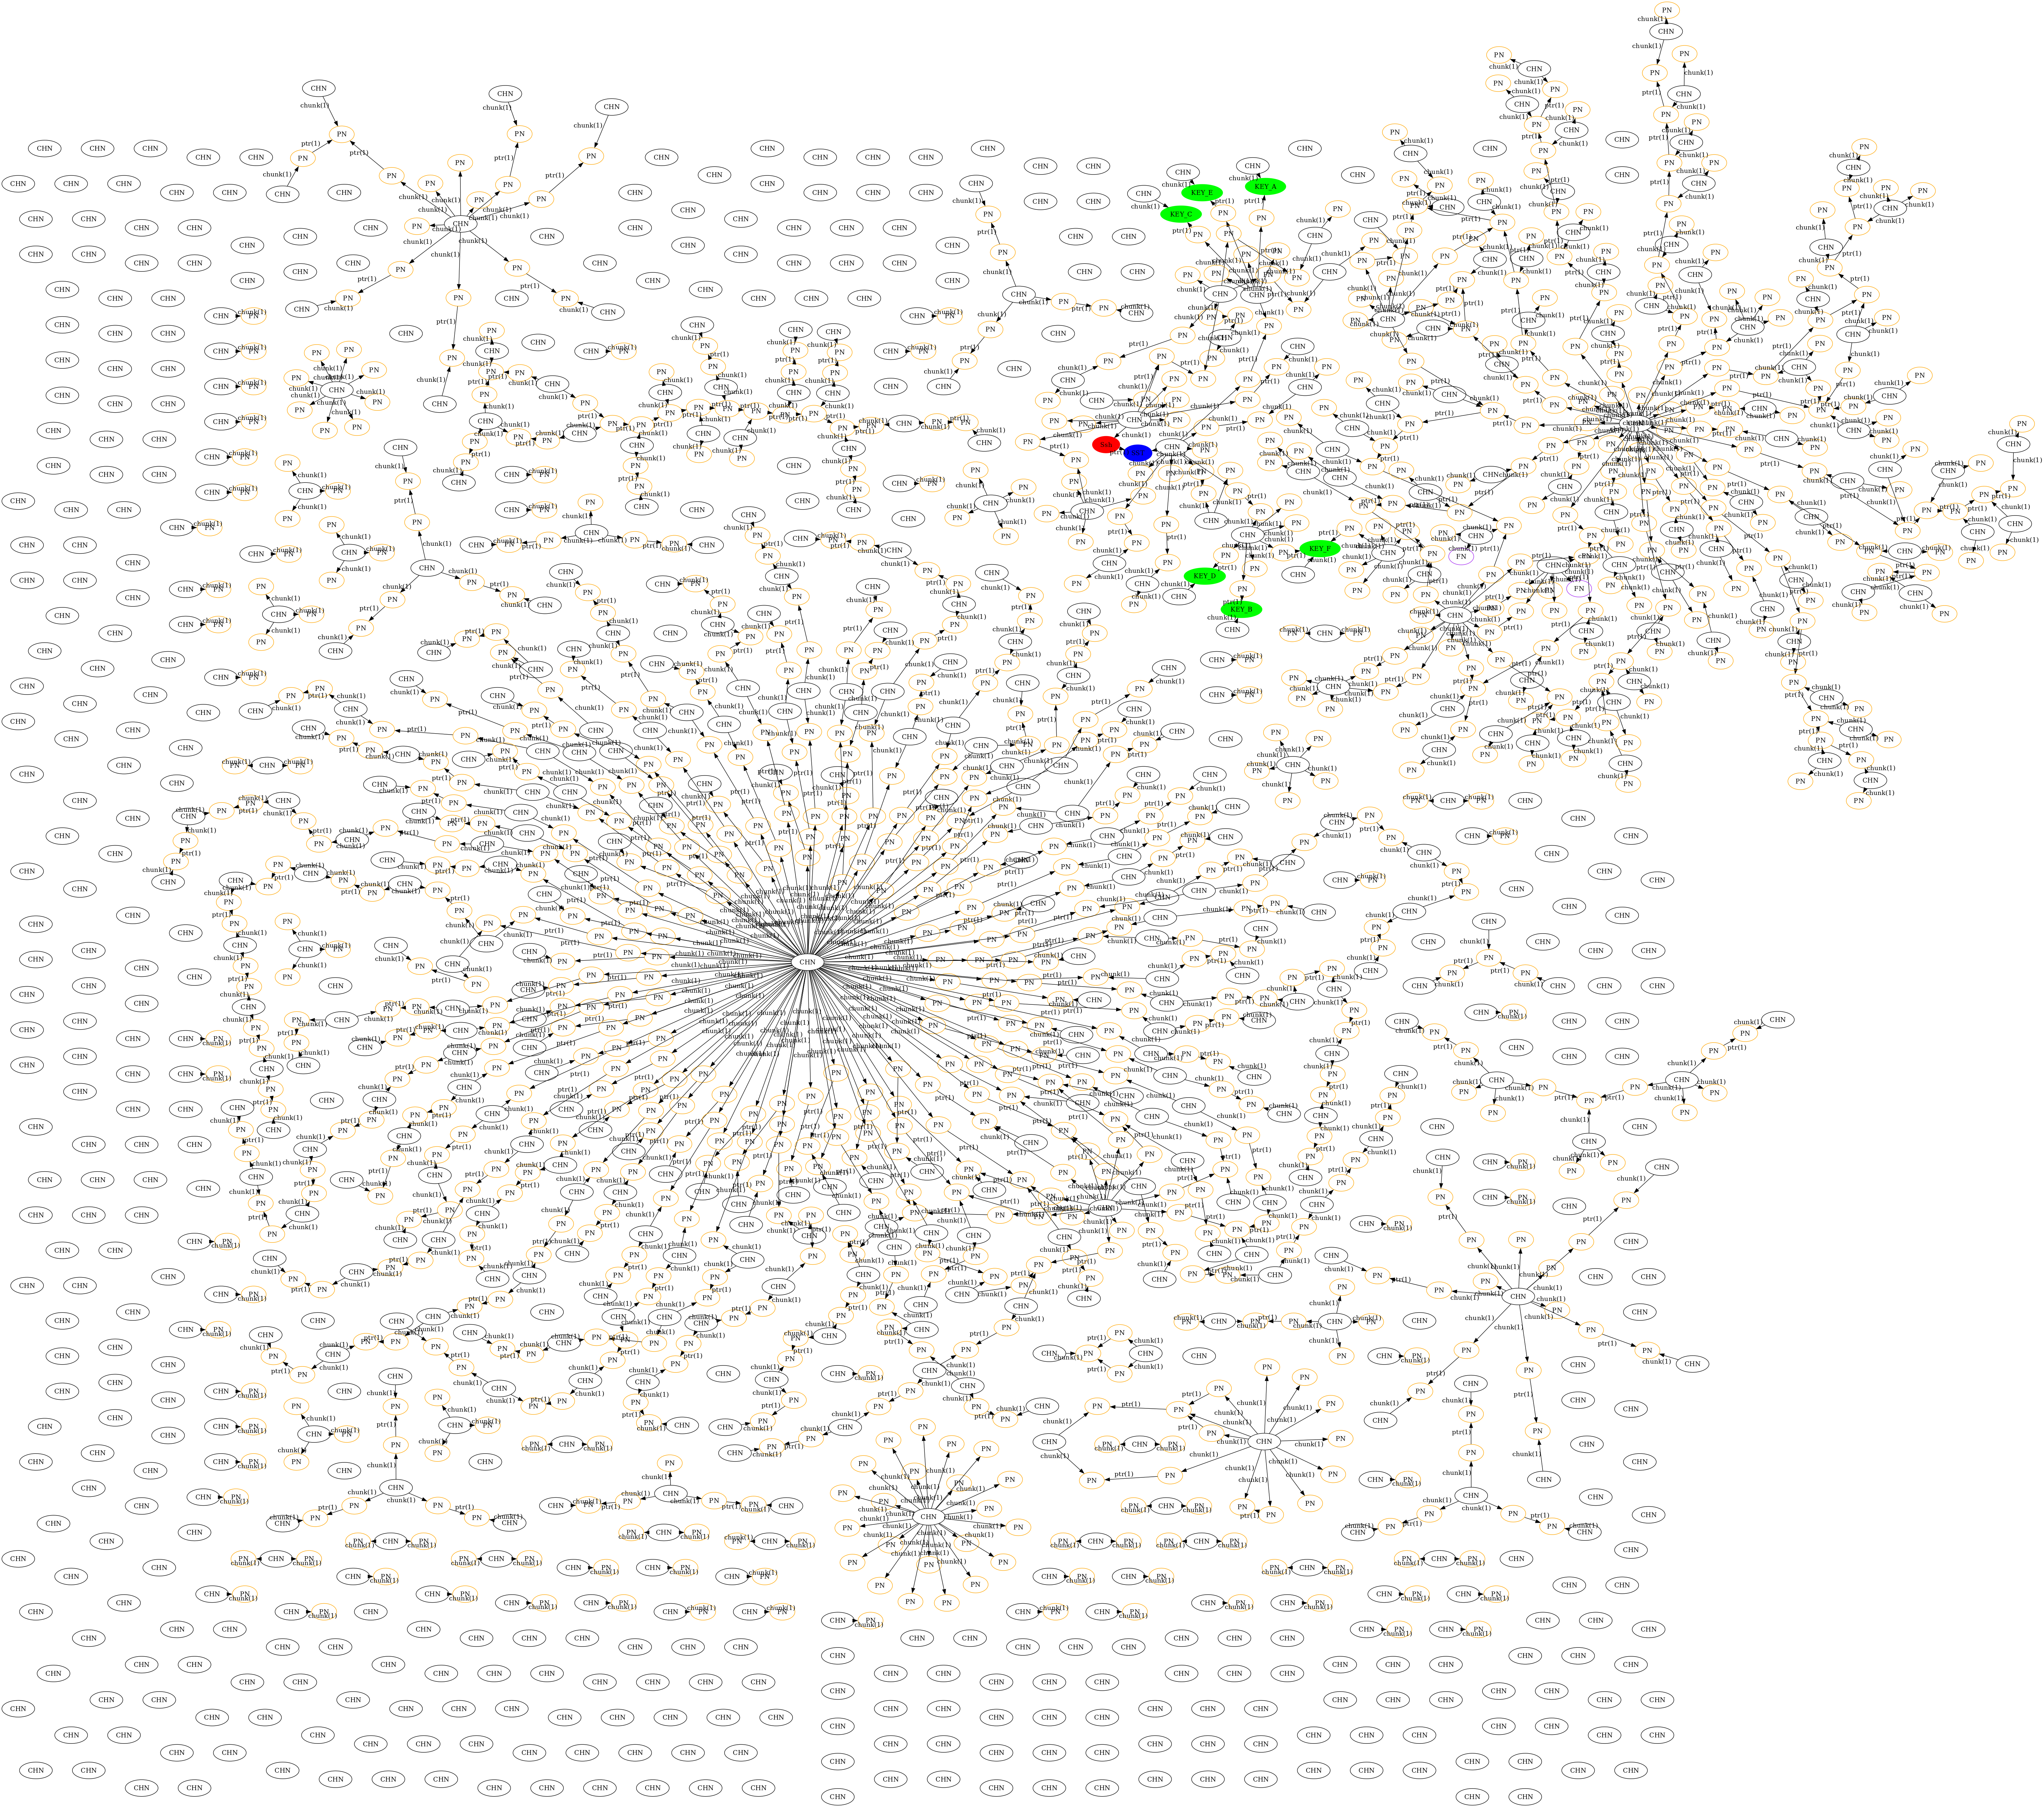
\includegraphics[width=0.9\textwidth]{img/graph_embeding/chunk_data_clean_27107-1643980590-heap.raw_dot_no_vn-sfdp.png}
            \caption{Graph example}
            \label{fig:graph_embedding:graph_example}
        \end{figure}

    \subsubsection{Graphs embedding}

        \paragraph{}Our next step is to uncover deeper insights and semantic understanding from our constructed graph, focusing on semantic embedding. This is the process through which we reshape our graph into a low-dimensional vector space, with each vector acting as a repository for a \gls{chunk}'s immediate neighborhood. Through this transformative journey, our aim is to forge vector representations that empower the application of cutting-edge machine learning techniques.

        \paragraph{}To create a concise yet informative representation, considering both structure-to-member and pointer-based connections, we meticulously count the number of \glspl{pointer} and \glspl{chunk} directly referencing a specific \gls{chunk}'s members. This initial count provides valuable insights into the \gls{chunk}'s immediate context. However, we doesn't stop there; we expand this representation by including counts of \glspl{pointer} and \glspl{chunk} pointing to those preceding nodes, allowing us to capture deeper layers of context. This recursive process continues until we reach a predetermined depth. Furthermore, we initiate a parallel analysis in reverse, meticulously tracing connections by following \glspl{pointer} from the initial \gls{chunk} to capture its children, recursively delving deeper until we reach the specified depth. We can see the algorithm here \ref{algo:embedding:generate_ancestor_children_embedding}. The result is a low-dimensional vector that intricately encodes the \gls{chunk}'s neighborhood, offering a comprehensive view of its relationships and contextual significance within the graph.

        \begin{algorithm}[H]
            \caption{Generate Ancestor/Children Embedding}
            \label{algo:embedding:generate_ancestor_children_embedding}
            \begin{algorithmic}
                \Function{GenerateNeighborsDTN}{$structure\_node, dir$}
                    \State $ancestor\_nodes \gets$ an empty set
                    \State $children \gets$ graph.neighbors\_directed($structure\_node, OUT$) \Comment{Get members of the structure}
                    \For{$child$ \textbf{in} $children$}
                        \State $ancestor\_nodes$.insert($child$)
                    \EndFor
                    \State $result \gets$ an empty list
                    \State $current\_nodes \gets$ an empty set
                    \For{$\_$ \textbf{in} $0$ \textbf{to} $DEPTH$}
                        \State $current\_nodes \gets$ $ancestor\_nodes$ \Comment{switch ancestor nodes and current nodes}
                        \State $ancestor\_nodes \gets$ an empty set
                        \State $nb\_dtn \gets 0$
                        \State $nb\_ptr \gets 0$
                        \For{$current\_node$ \textbf{in} $current\_nodes$}
                            \If{$node$ is DataStructureNode} \Comment{Update number of structures and pointers}
                                \State $nb\_dtn \gets nb\_dtn + 1$
                            \ElsIf{$node$ is PointerNode}
                                \State $nb\_ptr \gets nb\_ptr + 1$
                            \EndIf
                            \Comment{Get neighbors of the current node}
                            \For{$neighbor$ \textbf{in} graph.neighbors\_directed($current\_node, dir$)}
                                \State $ancestor\_nodes$.insert($neighbor$) \Comment{Add neighbors to the next ancestor nodes}
                            \EndFor
                        \EndFor
                        \State $result$.append($nb\_dtn$) \Comment{Add number of data structures}
                        \State $result$.append($nb\_ptr$) \Comment{Add number of pointers}
                    \EndFor
                    \State \textbf{return} $result$
                \EndFunction
            \end{algorithmic}
        \end{algorithm}
        
        \paragraph{}We can apply this algorithm to every \gls{chunk} within each graph, delving to a depth of 8, which produces an embedding of 32 units: 8 for ancestor \glspl{pointer}, 8 for ancestor \glspl{chunk}, 8 for child \glspl{pointer}, and 8 for child \glspl{chunk}. To accurately represent the \gls{chunk}'s neighborhood, it's crucial not to omit details about its members. Thus, we incorporate the count of \glspl{pointer} in the members and the \gls{chunk}'s dimensions. This results in a final embedding size of 34 - 32 for the neighborhood and an additional 2 for the \gls{chunk} size and \gls{pointer} count. However, there are inherent challenges with this embedding. It tends to get polluted by the value node, which often lacks significant meaning. Moreover, the relationships between the structures are intricate, and there's potential to represent them in a more straightforward manner, as show in the next section.

    \subsubsection{Updated graph}

        \paragraph{}Recognizing these challenges and the need for a clearer representation, we embarked on a series of refinements. Our approach focuses on enhancing the last graph by preserving the structure nodes and their interconnections via \glspl{pointer}. To simplify the visualization, we've decided to eliminate both the value nodes and the \gls{pointer} nodes. In addition, the relationships that previously connected the \gls{pointer} nodes to the value nodes will now link directly to the \gls{chunk} nodes, with the added detail of weighted edges. This strategy is driven by our aspiration to offer a more lucid graph, significantly reducing any extraneous noise, as show in the figure \ref{fig:graph_embedding:updated_graph}, the representation of the file \textit{14911-1644326802}.

        \begin{figure}[H]
            \centering
            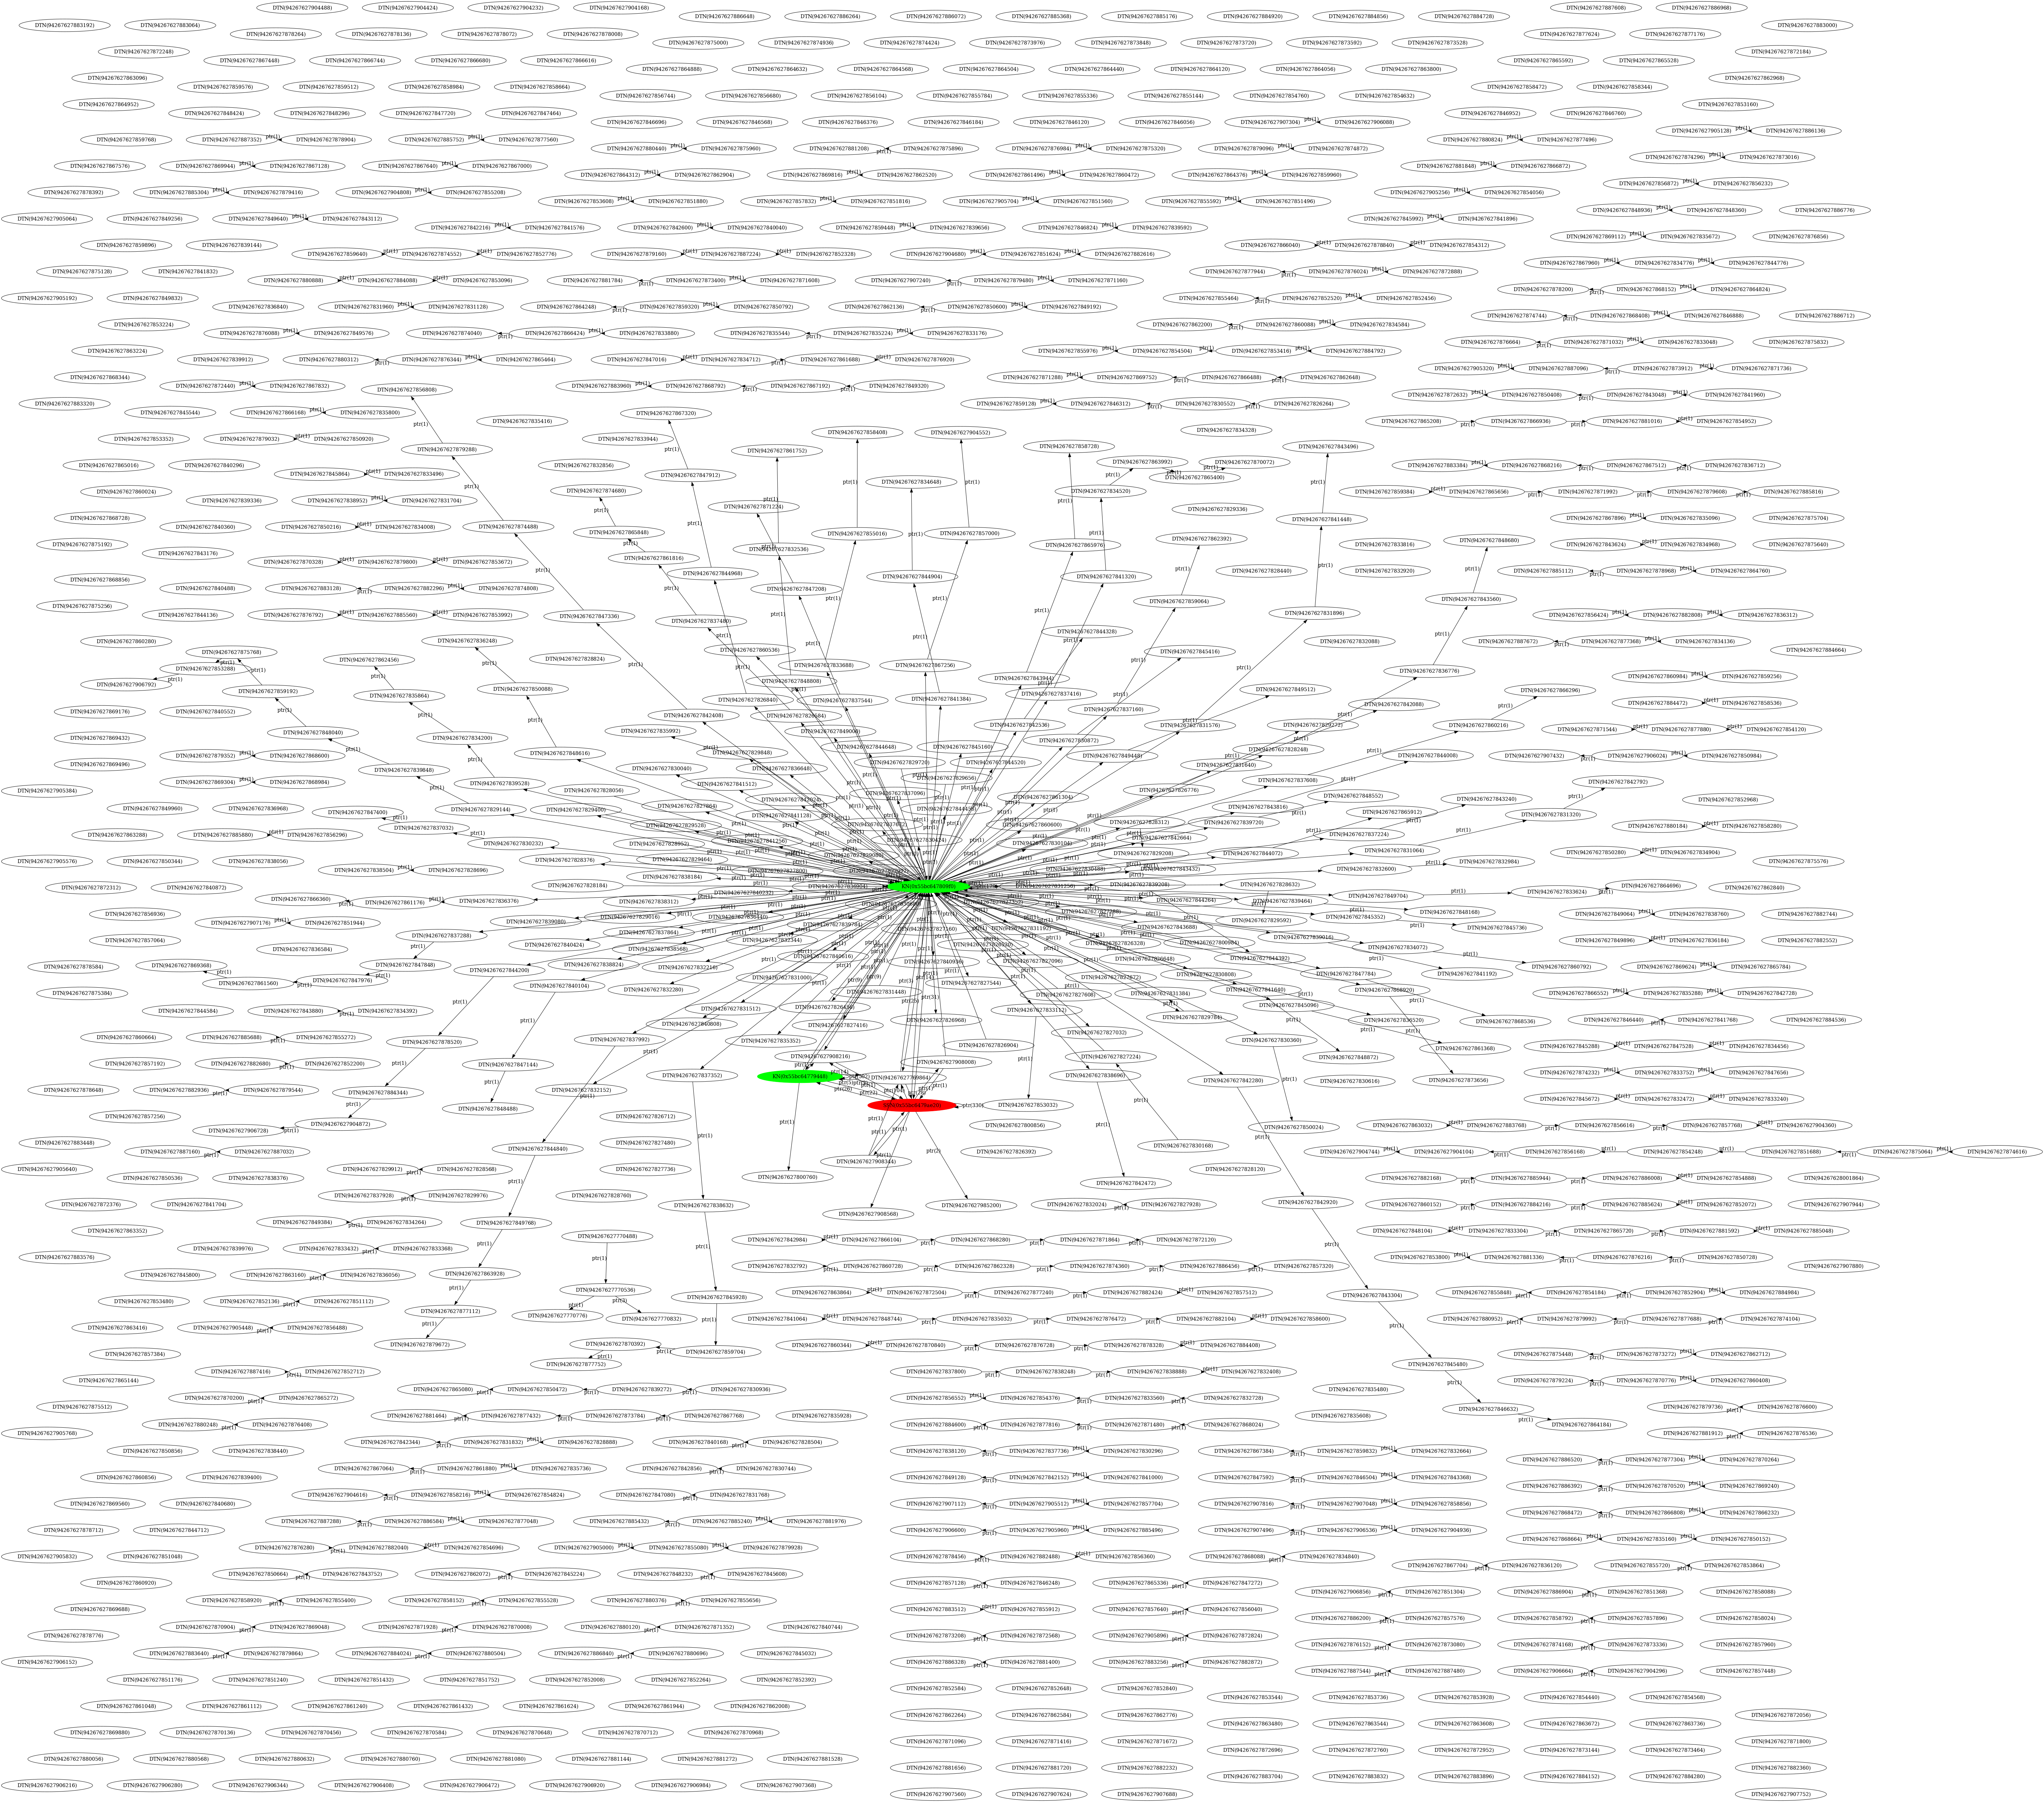
\includegraphics[width=0.9\textwidth]{img/graph_embeding/updated_graph_14911-1644326802-heap.png}
            \caption{Updated graph}
            \label{fig:graph_embedding:updated_graph}
        \end{figure}
        
\section{Embedding quality}\label{chap:embedding_quality}
\paragraph{}The quality of embeddings is paramount in machine learning, particularly when the objective is to identify specific \glspl{chunk} within data, such as the ones holding SSH keys. It becomes essential to juxtapose the performances of all embeddings in this context. An optimal embedding should proficiently discern the \glspl{chunk} containing SSH keys across the entire spectrum of openSSH use cases and for every conceivable key size. This necessitates the utilization of the complete dataset, with the training subset dedicated to model training and the validation subset for testing. Addressing this from a machine learning classification perspective, the random forest model, as elucidated in \ref{seq:background:some_ml_common_models}, emerges as the classifier of choice.

\paragraph{} To ensure fairness and comparability among the embeddings, we employ the Pearson correlation method \ref{seq:background:correlation_tests} to limit the selection to the top 8 correlations, thereby narrowing down our analysis to the most influential features. The dataset is notably imbalanced \ref{seq:background:imbalanced_data}, primarily stemming from the rarity of memory structures containing SSH keys, our specific target of interest, within the overall dataset. This rarity results in a significant class imbalance, where the majority of memory structures do not contain SSH keys. To counteract potential bias toward the majority class, we will implement random undersampling as a resampling strategy, particularly given our very large dataset. This approach will enable our model to accurately classify both majority and minority classes without being overwhelmed by the sheer volume of data. We will then employ a Random Forest model \ref{seq:background:machine_learning}, renowned for its robustness and suitability for high-dimensional data, to carry out the classification task. Our evaluation will rely on metrics such as precision, recall, F1 score, and others to identify the most effective representation for precise classification.

\subsection{Feature Selection and Dataset Challenges}

\paragraph{}In the quest for fairness across various embeddings and to circumvent the curse of dimensionality, it's imperative to maintain a uniform feature count across all embeddings. This is where feature engineering shines. The Pearson correlation method, elaborated in \ref{seq:background:correlation_tests}, is harnessed to meticulously select the 8 most salient features for each embedding. This count is a judicious compromise, ensuring the features are both succinct in number and information-rich. However, the dataset presents its own set of challenges. The instances of \glspl{chunk} containing SSH keys are dwarfed by those devoid of them, leading to a pronounced dataset imbalance. To counteract this skewness, the random undersampling technique, as referenced in \ref{seq:background:imbalanced_data}, is employed, when the dataset isn't filtered.

\subsection{Implementation and Evaluation Metrics}

\paragraph{}The implementation leans heavily on the scikit-learn library \cite{pedregosa_scikit-learn_2011} in Python, which provides the tools for the random forest classifier, Pearson correlation, and the random undersampling algorithm. Concurrently, the pandas library is indispensable for the efficient loading and manipulation of the dataset. Before diving into the analysis, it's crucial to ensure the embedding's integrity. This involves a rigorous sanity check, especially given the potential for corruption, such as NaN values. To guarantee the reproducibility of results, a consistent random seed is employed for both the random forest classifier and the random undersampling algorithm. For a comprehensive evaluation, the Pearson correlation matrix is preserved for each embedding. Moreover, a suite of metrics, including precision, recall, f1-score, AUC, and the confusion matrix (encompassing true positives, true negatives, false positives, and false negatives), is meticulously saved for every embedding.


\chapter{Results}\label{chap:results}

\paragraph{}In this thesis, we undertake a thorough investigation of data embeddings and their effectiveness in predicting SSH keys within OpenSSH memory dumps. The results are methodically structured, starting with Data Preprocessing, where we lay a solid foundation by preparing the data for in-depth analysis. We proceed to evaluate Deep Learning Models, analyzing their architecture and limitations. This is succeeded by Feature Engineering, where we meticulously refine our data to improve model accuracy. Through Clustering analysis, we explore and identify underlying patterns within the data. Ultimately, we employ Classification techniques to accurately predict and categorize SSH keys, thus demonstrating the practical implications and utility of our research. 
    

\section{Data Preprocessing}

\paragraph{}In the data preprocessing stage, we meticulously calculated each embedding four times, which included the deep learning models. This repetition was to test all combinations of the two filters—entropy and chunk size. The purpose of this thorough approach was to discern the effectiveness of each filter, both individually and in combination, providing us with a clearer understanding of their impact on the data and the subsequent results. The different datasets used are detailed in Section \ref{sec:annexe:all_dataset}. The dataset codes are explained in the following table~\ref{tab:results:dataset_codes}:

\begin{table}[ht]
    \centering
    \begin{tabular}{|p{0.3\linewidth}|p{0.6\linewidth}|}
    \hline
    Dataset Code & Meaning \\ 
    \hline
    value\_node\_embedding & First graph embedding, with all nodes~\ref{sec:embedding:first_graph} \\ \hline
    chunk\_top\_vn\_semantic\_embedding & First graph embedding, keeping only the first block of each chunk~\ref{sec:embedding:first_graph_only_first_block} \\ \hline
    chunk\_semantic\_embedding & Second graph embedding~\ref{sec:embedding:updated_graph} \\ \hline
    chunk\_statistic\_embedding & Statistical embedding~\ref{sec:embedding:statistical} \\ \hline
    chunk\_start\_bytes\_embedding & Start bytes embedding~\ref{sec:embedding:trim_method} \\ \hline
    chunk\_extraction & Raw byte extraction with filters, to be fed into the deep learning model\\ \hline
    \end{tabular}
    \caption{Meanings of Dataset Codes}
    \label{tab:results:dataset_codes}
\end{table}


\section{Deep Learning Models}

\paragraph{}The exploration of hyperparameters is documented in Section \ref{sec:annexes:deep_learning_hyperparameters}. During our experiments, we encountered instances where some models either ran out of memory, as noted in Sections \ref{sec:annexe:out_of_memory_instances_classifications} and \ref{sec:annexe:out_of_memory_instances_clustering}, or experienced timeouts, detailed in Section \ref{sec:annexe:timeout_instances}. Consequently, our discussion will be confined to the results yielded by the models that successfully completed their runs.

\paragraph{}Within the cohort of operational deep learning models, we endeavored to identify the most proficient instance for each algorithm, whether it was Transformers or Word2Vec. However, we encountered a scarcity of successful instances, which impeded our ability to conclusively determine the optimal hyperparameters or to fully understand their impact on the classification metrics. It was observed that instances with a larger word size and a reduced embedding dimension were more likely to succeed, presumably due to the decreased computational load they required.

\section{Feature Engineering}
\paragraph{}During our feature engineering phase, we encountered a challenge that led to the elimination of certain embeddings. This was due to the invariance observed in the columns, an issue that is elaborated upon in Section \ref{sec:annexe:feature_engineering_fails}. The specific embedding that was rendered ineffective and subsequently removed was the semantic embedding of the first graph, as discussed in Section \ref{sec:embedding:graph_embedding}. This elimination was necessary regardless of whether the filter on the first block of each chunk was applied. The primary shortcoming of this embedding was its inability to generate a sufficient number of ancestors to provide useful information. This inadequacy arose because only a minor segment of the value nodes were being pointed to by pointers, which significantly limited the utility of the embedding. In contrast, the second graph managed to compress the information effectively, thereby validating the semantic embedding by conveying more meaningful data for each node.

\paragraph{}The instances that successfully passed the feature engineering stage are meticulously recorded in Section \ref{sec:annexe:feature_engineering_results}. Here, the eight most significant columns are identified.

\section{Clustering}
\paragraph{}In the clustering phase of our analysis, we categorized the data into distinct groups: label 1 for SSH keys, label 2 for "ssh\_struct", label 4 for "session\_state\_struct", and label 0 for the remainder. The detailed outcomes of this clustering are presented in appendix \ref{sec:annexe:clustering_results}. Our examination revealed that the majority of clusters did not exhibit discernible patterns. However, certain datasets, such as those represented by chunk\_start\_bytes\_embedding (23) in Table \ref{tab:23_single_instance_clustering_results} and chunk\_statistic\_embedding (18) in Table \ref{tab:18_single_instance_clustering_results}, maintained a ratio of labels similar to that of the original dataset.


\paragraph{}Interestingly, the clusters derived from deep learning models typically displayed an even distribution of labels, with approximately one quarter of the data falling into each category. An exception to this trend was observed in the Word2Vec 3 Clustering Results on dataset 25 (with chunk size filter), as shown in Table \ref{tab:25_word2vec_3_clustering_results}, which consisted of three clusters with seemingly random label proportions.

\paragraph{}The results from the clustering analysis were not entirely definitive, indicating that there is substantial room for improvement in the methodology. Future efforts in this area would benefit from a more refined approach to enhance the clarity and significance of the clustering outcomes.

\section{Classification}

\paragraph{}The classification results of our study, detailed in appendix \ref{sec:annexe:classification_results}, yielded highly promising results. The performance of various instances, particularly in terms of accuracy, is depicted in the graphical representation found in Figure \ref{fig:results:best_accuracy_instances}, which ranks the instances from best to worst.

\begin{figure}[ht]
    \centering
    \includegraphics[width=0.6\textwidth]{img/annexes/Best Accuracy (by instances).png}
    \caption{Metrics for the best instances (accuracy)}
    \label{fig:results:best_accuracy_instances}
\end{figure}

\paragraph{}The two top-performing instances, both utilizing chunk\_start\_bytes\_embedding, achieved remarkable accuracy scores of 99.90\% with the chunk size filter~\ref{tab:21_single_instance_classifiers_results} and 99.84\% without the filter~\ref{tab:20_single_instance_classifiers_results}. Following closely was chunk\_semantic\_embedding with the chunk size filter, securing an accuracy of 99.70\%~\ref{tab:9_single_instance_classifiers_results}. Notably, the first deep learning model to make an appearance in the ranking was a Word2Vec model, which, with both entropy and chunk size filters applied, attained an accuracy of 98.79\%, placing it sixth overall~\ref{tab:27_word2vec_3_classifiers_results}.

\paragraph{}When focusing on recall for label 1, the best instance was chunk\_start\_bytes\_embedding without any filter, achieving a perfect recall of 100\%~\ref{tab:20_single_instance_classifiers_results}, as shown in Figure \ref{fig:results:best_label_1_recall_instances}. The second-best was again chunk\_start\_bytes\_embedding, this time with both entropy and chunk size filters, achieving a recall of 99.99553\%~\ref{tab:23_single_instance_classifiers_results}. The first deep learning model, a Word2Vec instance with both filters, ranked third with a recall of 99.95\%.

\begin{figure}[ht]
    \centering
    \includegraphics[width=0.6\textwidth]{img/annexes/Best 1.0 Recall (by instances).png}
    \caption{Metrics for the best instances (Label 1 recall)}
    \label{fig:results:best_label_1_recall_instances}
\end{figure}

\paragraph{}As for precision on label 1, the highest achievement was recorded by chunk\_statistic\_embedding with the entropy filter, which reached a precision of 96.86\%~\ref{tab:18_single_instance_classifiers_results}, as illustrated in Figure \ref{fig:results:best_label_1_precision_instances}. The second-highest precision came from a Word2Vec deep learning model with both entropy and chunk size filters, scoring 95.19\%.

\begin{figure}[ht]
    \centering
    \includegraphics[width=0.6\textwidth]{img/annexes/Best 1.0 Precision (by instances).png}
    \caption{Metrics for the best instances (Label 1 precision)}
    \label{fig:results:best_label_1_precision_instances}
\end{figure}


\chapter{Discussion}\label{chap:discussion}




\section{Limits}

\paragraph{}This study, while comprehensive, acknowledges several limitations that warrant mention. Within the realm of data embedding, a notable constraint is the necessity to deactivate the entropy filter during the validation phase to prevent the inadvertent exclusion of keys. Additionally, the NLP models, such as Word2Vec and transformers, are highly sensitive to hyperparameter tuning. Due to time constraints, we have explored only a limited subset of these parameters, which may impact the robustness of our findings.

\paragraph{}Memory consumption poses another significant challenge, particularly for NLP models and some simpler embedding techniques. The computational resources available for this study, specifically the server with 516 GB of RAM, restricted our ability to process some of the more demanding models.

\paragraph{}In the evaluation of embedding performance, the decision to limit features to eight was arbitrary and could have been adjusted to better suit the characteristics of each embedding. While the Pearson algorithm was chosen for its ease of implementation, more sophisticated dimensionality reduction techniques, such as PCA, might have yielded more nuanced insights. Furthermore, the exclusion of time as a factor in the analysis was a deliberate choice to maintain consistency across models. However, time is a critical element in practical applications, such as SSH key detection, and should be considered in future evaluations.

\paragraph{}The section on embedding coherence also presents its own set of challenges. Clustering, while a powerful tool, is difficult to interpret and optimize, requiring careful tuning of numerous hyperparameters. The time and memory demands of clustering have limited the depth of exploration in this thesis. Consequently, the results obtained were not as robust as desired, and the methods employed to manage data volume, such as random undersampling, were not ideal.

\section{Future Work}

\paragraph{}Looking ahead, there is ample opportunity for further research and enhancement in several areas. The embedding techniques could benefit from the application of more sophisticated or varied NLP models, along with extensive hyperparameter tuning. Improvements in the performance evaluation of embeddings could be achieved through the use of more advanced dimensionality reduction algorithms and a more detailed examination of processing time to better differentiate between models.

\paragraph{}The exploration of embedding coherence in this thesis is merely an initial foray. Significant improvements could be realized with a more refined approach to dataset preparation and further tuning of clustering algorithms. As such, these areas present fruitful avenues for future research and development.



\chapter{Conclusion}\label{chap:conclusion}

\paragraph{}In conclusion, this Master's thesis has provided a comprehensive survey of various embedding techniques for the classification of SSH keys in OpenSSH memory dumps. The study has uncovered that simple embedding techniques, such as the trim method and statistical approaches, yield highly effective results when applied to this specific dataset. Additionally, NLP techniques like Word2Vec and Transformers have shown promising outcomes, although they require further refinement through hyperparameter tuning to reach their full potential.

\paragraph{}While coherence testing has not been conclusively demonstrated, the classification results have been exceptionally positive, indicating the practical value of the research. However, there remains a substantial scope for future work. This includes measuring the time efficiency of the embedding processes, extensive hyperparameter optimization, exploration of additional NLP techniques, and more rigorous coherence testing. These areas present exciting opportunities for further research and development in the field of digital forensics and cybersecurity.

\chapter{Ressources}\label{chap:ressources}

TODO : make transition

\section{hardware}
\paragraph{}My primary workstation is an \textit{Aspire 5} laptop, equipped with:
\begin{itemize}
    \item \textbf{CPU:} 11th Gen Intel i5-1135G7 (8) @ 4.200GHz 
    \item \textbf{GPU:} Intel TigerLake-LP GT2 [Iris Xe Graphics]
    \item \textbf{Memory:} 16GB
\end{itemize}
\paragraph{}However, this laptop, despite its decent specifications, proved inadequate for processing the entire dataset. Simple machine learning experiments using a Python script would have stretched over a week. Even when we transitioned to more optimized Rust programs, the processing time exceeded 10 hours. While we managed to run minor tasks and scripts on this laptop, the bulk of the experiments necessitated a more powerful server.

\paragraph{}Recognizing this need, we was granted access to a high-performance development server in the later stages of the thesis, around August 2023. The server, an \textit{AS-4124GS-TNR}, boasts the following specifications:
\begin{itemize}
    \item \textbf{CPU:} 2x AMD EPYC 7662 (256) @ 2.000GHz
    \item \textbf{GPU:} NVIDIA Geforce RTX 3090 Ti
    \item \textbf{RAM:} 512GB DDR4 3200MHz
\end{itemize}
\paragraph{}Operating on \textit{Ubuntu 20.04.6 LTS}, this server became the primary platform for the machine learning experiments, given its superior computational capabilities compared to the \textit{Aspire 5} laptop. This invaluable resource was generously provided by the Department of Computer Science at \textit{Universität Passau}, particularly under the guidance of the Chair of Data Science led by Prof. Dr. Michael Granitzer. I extend my sincere appreciation for their unwavering support.



%%%%%%%%%%%%%%%%%%%%%%%%%%%%%%%%%%%%%%%%%%%%%%%%%%%%%%%%%%%%%%%%%%%%%%%%%%%%%%%%%%%%%%%%%
\newpage
% -- Appendix (optional)
\begin{appendices}
    % !TeX spellcheck = en\_US
% !TeX encoding = UTF-8
\chapter{Code}

\chapter{Math}

\chapter{Dataset}

    \section{Dataset cleaning results}\label{sec:annexes:dataset_cleaning_results}
        \paragraph{}The empty folder for the training part of the dataset after cleaning are : 
        \begin{itemize}
            \item Use case: port-forwarding, OpenSSH version: V\_8\_0\_P1, Key size: 64
            \item Use case: port-forwarding, OpenSSH version: V\_8\_0\_P1, Key size: 32
            \item Use case: port-forwarding, OpenSSH version: V\_7\_8\_P1, Key size: 16
            \item Use case: port-forwarding, OpenSSH version: V\_7\_8\_P1, Key size: 64
            \item Use case: port-forwarding, OpenSSH version: V\_7\_8\_P1, Key size: 32
            \item Use case: scp, OpenSSH version: V\_8\_0\_P1, Key size: 64
            \item Use case: scp, OpenSSH version: V\_8\_0\_P1, Key size: 32
            \item Use case: scp, OpenSSH version: V\_7\_8\_P1, Key size: 64
            \item Use case: scp, OpenSSH version: V\_7\_8\_P1, Key size: 32
            \item Use case: basic, OpenSSH version: V\_8\_7\_P1, Key size: 16
            \item Use case: basic, OpenSSH version: V\_8\_7\_P1, Key size: 64
            \item Use case: basic, OpenSSH version: V\_8\_7\_P1, Key size: 32
            \item Use case: basic, OpenSSH version: V\_8\_8\_P1, Key size: 16
            \item Use case: basic, OpenSSH version: V\_8\_8\_P1, Key size: 64
            \item Use case: basic, OpenSSH version: V\_8\_8\_P1, Key size: 32
            \item Use case: basic, OpenSSH version: V\_7\_0\_P1, Key size: 16
            \item Use case: basic, OpenSSH version: V\_7\_0\_P1, Key size: 64
            \item Use case: basic, OpenSSH version: V\_7\_0\_P1, Key size: 32
            \item Use case: basic, OpenSSH version: V\_6\_8\_P1, Key size: 16
            \item Use case: basic, OpenSSH version: V\_6\_8\_P1, Key size: 64
            \item Use case: basic, OpenSSH version: V\_6\_8\_P1, Key size: 32
            \item Use case: basic, OpenSSH version: V\_6\_2\_P1, Key size: 16
            \item Use case: basic, OpenSSH version: V\_6\_2\_P1, Key size: 24
            \item Use case: basic, OpenSSH version: V\_6\_2\_P1, Key size: 32
            \item Use case: basic, OpenSSH version: V\_6\_0\_P1, Key size: 16
            \item Use case: basic, OpenSSH version: V\_6\_0\_P1, Key size: 24
            \item Use case: basic, OpenSSH version: V\_6\_0\_P1, Key size: 32
            \item Use case: basic, OpenSSH version: V\_8\_1\_P1, Key size: 16
            \item Use case: basic, OpenSSH version: V\_8\_1\_P1, Key size: 64
            \item Use case: basic, OpenSSH version: V\_8\_1\_P1, Key size: 32
            \item Use case: basic, OpenSSH version: V\_6\_1\_P1, Key size: 16
            \item Use case: basic, OpenSSH version: V\_6\_1\_P1, Key size: 24
            \item Use case: basic, OpenSSH version: V\_6\_1\_P1, Key size: 32
            \item Use case: basic, OpenSSH version: V\_7\_2\_P1, Key size: 16
            \item Use case: basic, OpenSSH version: V\_7\_2\_P1, Key size: 64
            \item Use case: basic, OpenSSH version: V\_7\_2\_P1, Key size: 32
            \item Use case: basic, OpenSSH version: V\_8\_0\_P1, Key size: 16
            \item Use case: basic, OpenSSH version: V\_8\_0\_P1, Key size: 64
            \item Use case: basic, OpenSSH version: V\_8\_0\_P1, Key size: 32
            \item Use case: basic, OpenSSH version: V\_6\_3\_P1, Key size: 16
            \item Use case: basic, OpenSSH version: V\_6\_3\_P1, Key size: 24
            \item Use case: basic, OpenSSH version: V\_6\_3\_P1, Key size: 32
            \item Use case: basic, OpenSSH version: V\_6\_9\_P1, Key size: 16
            \item Use case: basic, OpenSSH version: V\_6\_9\_P1, Key size: 64
            \item Use case: basic, OpenSSH version: V\_6\_9\_P1, Key size: 32
            \item Use case: basic, OpenSSH version: V\_7\_1\_P1, Key size: 16
            \item Use case: basic, OpenSSH version: V\_7\_1\_P1, Key size: 64
            \item Use case: basic, OpenSSH version: V\_7\_1\_P1, Key size: 32
            \item Use case: basic, OpenSSH version: V\_7\_9\_P1, Key size: 16
            \item Use case: basic, OpenSSH version: V\_7\_9\_P1, Key size: 64
            \item Use case: basic, OpenSSH version: V\_7\_9\_P1, Key size: 32
            \item Use case: basic, OpenSSH version: V\_6\_7\_P1, Key size: 16
            \item Use case: basic, OpenSSH version: V\_6\_7\_P1, Key size: 24
            \item Use case: basic, OpenSSH version: V\_6\_7\_P1, Key size: 32
            \item Use case: basic, OpenSSH version: V\_7\_8\_P1, Key size: 16
            \item Use case: basic, OpenSSH version: V\_7\_8\_P1, Key size: 64
            \item Use case: basic, OpenSSH version: V\_7\_8\_P1, Key size: 32
            \item Use case: client, OpenSSH version: V\_8\_0\_P1, Key size: 16
            \item Use case: client, OpenSSH version: V\_8\_0\_P1, Key size: 64
            \item Use case: client, OpenSSH version: V\_8\_0\_P1, Key size: 32
            \item Use case: client, OpenSSH version: V\_7\_8\_P1, Key size: 16
            \item Use case: client, OpenSSH version: V\_7\_8\_P1, Key size: 64
            \item Use case: client, OpenSSH version: V\_7\_8\_P1, Key size: 32
        \end{itemize}

        \paragraph{}The empty folder for the validation part of the dataset after cleaning are : 
        \begin{itemize}
            \item Use case: port-forwarding, OpenSSH version: V\_8\_0\_P1, Key size: 64
            \item Use case: port-forwarding, OpenSSH version: V\_8\_0\_P1, Key size: 32
            \item Use case: port-forwarding, OpenSSH version: V\_7\_8\_P1, Key size: 16
            \item Use case: port-forwarding, OpenSSH version: V\_7\_8\_P1, Key size: 64
            \item Use case: port-forwarding, OpenSSH version: V\_7\_8\_P1, Key size: 32
            \item Use case: scp, OpenSSH version: V\_8\_0\_P1, Key size: 64
            \item Use case: scp, OpenSSH version: V\_8\_0\_P1, Key size: 32
            \item Use case: scp, OpenSSH version: V\_7\_8\_P1, Key size: 64
            \item Use case: scp, OpenSSH version: V\_7\_8\_P1, Key size: 32
            \item Use case: basic, OpenSSH version: V\_8\_7\_P1, Key size: 16
            \item Use case: basic, OpenSSH version: V\_8\_7\_P1, Key size: 64
            \item Use case: basic, OpenSSH version: V\_8\_7\_P1, Key size: 32
            \item Use case: basic, OpenSSH version: V\_8\_8\_P1, Key size: 16
            \item Use case: basic, OpenSSH version: V\_8\_8\_P1, Key size: 64
            \item Use case: basic, OpenSSH version: V\_8\_8\_P1, Key size: 32
            \item Use case: basic, OpenSSH version: V\_7\_0\_P1, Key size: 16
            \item Use case: basic, OpenSSH version: V\_7\_0\_P1, Key size: 64
            \item Use case: basic, OpenSSH version: V\_7\_0\_P1, Key size: 32
            \item Use case: basic, OpenSSH version: V\_6\_8\_P1, Key size: 16
            \item Use case: basic, OpenSSH version: V\_6\_8\_P1, Key size: 64
            \item Use case: basic, OpenSSH version: V\_6\_8\_P1, Key size: 32
            \item Use case: basic, OpenSSH version: V\_6\_2\_P1, Key size: 16
            \item Use case: basic, OpenSSH version: V\_6\_2\_P1, Key size: 24
            \item Use case: basic, OpenSSH version: V\_6\_2\_P1, Key size: 32
            \item Use case: basic, OpenSSH version: V\_6\_0\_P1, Key size: 16
            \item Use case: basic, OpenSSH version: V\_6\_0\_P1, Key size: 24
            \item Use case: basic, OpenSSH version: V\_6\_0\_P1, Key size: 32
            \item Use case: basic, OpenSSH version: V\_8\_1\_P1, Key size: 16
            \item Use case: basic, OpenSSH version: V\_8\_1\_P1, Key size: 64
            \item Use case: basic, OpenSSH version: V\_8\_1\_P1, Key size: 32
            \item Use case: basic, OpenSSH version: V\_6\_1\_P1, Key size: 16
            \item Use case: basic, OpenSSH version: V\_6\_1\_P1, Key size: 24
            \item Use case: basic, OpenSSH version: V\_6\_1\_P1, Key size: 32
            \item Use case: basic, OpenSSH version: V\_7\_2\_P1, Key size: 16
            \item Use case: basic, OpenSSH version: V\_7\_2\_P1, Key size: 64
            \item Use case: basic, OpenSSH version: V\_7\_2\_P1, Key size: 32
            \item Use case: basic, OpenSSH version: V\_8\_0\_P1, Key size: 16
            \item Use case: basic, OpenSSH version: V\_8\_0\_P1, Key size: 64
            \item Use case: basic, OpenSSH version: V\_8\_0\_P1, Key size: 32
            \item Use case: basic, OpenSSH version: V\_6\_3\_P1, Key size: 16
            \item Use case: basic, OpenSSH version: V\_6\_3\_P1, Key size: 24
            \item Use case: basic, OpenSSH version: V\_6\_3\_P1, Key size: 32
            \item Use case: basic, OpenSSH version: V\_6\_9\_P1, Key size: 16
            \item Use case: basic, OpenSSH version: V\_6\_9\_P1, Key size: 64
            \item Use case: basic, OpenSSH version: V\_6\_9\_P1, Key size: 32
            \item Use case: basic, OpenSSH version: V\_7\_1\_P1, Key size: 16
            \item Use case: basic, OpenSSH version: V\_7\_1\_P1, Key size: 64
            \item Use case: basic, OpenSSH version: V\_7\_1\_P1, Key size: 32
            \item Use case: basic, OpenSSH version: V\_7\_9\_P1, Key size: 16
            \item Use case: basic, OpenSSH version: V\_7\_9\_P1, Key size: 64
            \item Use case: basic, OpenSSH version: V\_7\_9\_P1, Key size: 32
            \item Use case: basic, OpenSSH version: V\_6\_7\_P1, Key size: 16
            \item Use case: basic, OpenSSH version: V\_6\_7\_P1, Key size: 24
            \item Use case: basic, OpenSSH version: V\_6\_7\_P1, Key size: 32
            \item Use case: basic, OpenSSH version: V\_7\_8\_P1, Key size: 16
            \item Use case: basic, OpenSSH version: V\_7\_8\_P1, Key size: 64
            \item Use case: basic, OpenSSH version: V\_7\_8\_P1, Key size: 32
            \item Use case: client, OpenSSH version: V\_8\_0\_P1, Key size: 16
            \item Use case: client, OpenSSH version: V\_8\_0\_P1, Key size: 64
            \item Use case: client, OpenSSH version: V\_8\_0\_P1, Key size: 32
            \item Use case: client, OpenSSH version: V\_7\_8\_P1, Key size: 16
            \item Use case: client, OpenSSH version: V\_7\_8\_P1, Key size: 32
        \end{itemize}
\end{appendices}

% glossary and acronyms
\newpage
% \printglossary[type=\acronymtype, title=Acronymes]
% \printglossary[title=Glossaire]
\printglossary[type=\acronymtype]

\printglossary

% biblio
\newpage
\printbibliography[
    heading=bibintoc,
    category=cited,
    title={References}
]

% uncited references (bibliography)
% https://tex.stackexchange.com/questions/6967/how-to-split-bibliography-into-works-cited-and-works-not-cited
\printbibliography[
    notcategory=cited,
    heading=bibintoc,
    title={Additional bibliography},
]

% -- Eidesstattliche Erklärung (= Affadavit)
% !TeX spellcheck = de_DE
% !TeX encoding = UTF-8

\section*{Eidesstattliche Erkl\"arung}

	Hiermit versichere ich, dass ich diese Masterarbreit selbstst\"andig und ohne Benutzung anderer als der angegebenen Quellen und Hilfsmittel angefertigt habe und alle Ausf\"uhrungen, die w\"ortlich oder sinngem\"a\ss{} übernommen wurden, als solche gekennzeichnet sind, sowie, dass ich die Masterarbreit ~in gleicher oder \"ahnlicher Form noch keiner anderen Pr\"ufungsbeh\"orde vorgelegt habe.

	\vspace{3cm}

	Passau, \today

	\vspace{2cm}

	\parbox{8cm}{
		\hrule \strut \theauthor
	}



\restoregeometry
\end{document}